\documentclass[onecolumn,doublespacing]{risa}

\usepackage[figuresright]{rotating}
\usepackage{afterpage}
\usepackage{enumitem}
\usepackage{moreverb,url}
\PassOptionsToPackage{hyphens}{url}\usepackage{hyperref}
\usepackage[american]{babel}
\usepackage{csquotes}
\usepackage[
    style=apa,
    backend=biber,
    sortcites=true,
    maxcitenames=2,
    sorting=nyt,
%    isbn=false,
%    url=false,
%    doi=false,
%    eprint=false,
    hyperref=false,
    backref=false,
%    firstinits=false,
]{biblatex}
\let \citeNP \cite
\let \citeA \textcite
\let \cite \parencite

\makeatletter
\AtEveryCitekey{\ifnameundef{shortauthor}{}{\def\cbx@apa@ifnamesaved{\@firstoftwo}}}
\makeatother


\DeclareLanguageMapping{american}{american-apa}

\bibliography{references}


\begin{document}

\jvol{}
\jnum{}
\pubyear{}

\doi{}
\copyright{}
\issnyear{}

\title{Reframing Resilience: Equitable Access to Essential Services}

\author[Logan]{Tom M Logan,$^{1}$\affiliation{Civil and Natural Resources Engineering, University of Canterbury, New Zealand, tom.logan@canterbury.ac.nz}
%
Seth D Guikema$^{2}$\affiliation{Industrial and Operations Engineering, University of Michigan, Ann Arbor, USA}
}

\maketitle
\newpage

\section*{Abstract}
We urgently need to put the concept of resilience into practice if we are to prepare our communities for climate change and exacerbated natural hazards.
Yet, despite the extensive discussion surrounding community resilience, operationalizing the concept remains challenging. 
The dominant approaches for assessing resilience focus on either evaluating community characteristics or infrastructure functionality. 
While both remain useful, they have several limitations to their ability to provide actionable insight.
More importantly, the current conceptualizations do not consider essential services or how access is impaired by hazards. 
We argue that people need access to services such as food, education, healthcare, and cultural amenities, in addition to water, power, sanitation, and communications, to get back some semblance of normal life.
Providing equitable access to these types of services and quickly restoring that access following a disruption is paramount to community resilience. 
We propose a new conceptualization of community resilience that is based on access to essential services.
This reframing of resilience facilitates a new measure of resilience that is spatially explicit and operational. 
Using two illustrative examples from the impacts of Hurricanes Florence and Michael, we demonstrate how decision-makers and planners can use this framework to visualize the effect of a hazard and quantify resilience-enhancing interventions. 
This ``equitable access to essentials'' approach to community resilience integrates with spatial planning, and will enable communities not only to ``bounce back" from a disruption, but to ``bound forward'' and improve the resilience and quality of life for all residents.

\textbf{Keywords:} Community resilience; Natural hazards; Social justice; Spatial planning; Climate change
\newpage

\section{Introduction}
Resilience is a concept around which many people center discussion of community well-being over time in the face of risk.
It is used to describe the capacity of a system to withstand, prepare for, recover from, and adapt or transform following hazards \cite{Bene2012-mx, Meerow2016-definingRes, GillespieMarthaler2019-ak}.
In the face of such expectation, the concept of resilience has ballooned. 
The result is that the measure of resilience is hotly contested \cite{Levine2014-je, Woolf2016-vm, Klein2003-lc}.
However, measuring resilience will further enable communities to improve their resilience \cite{Cutter2013-hq}.
Additionally, measuring resilience will help us to evaluate synergies and trade-offs of interventions, and better understand and manage the risk from hazards.
Therefore, we urgently need to find appropriate and actionable measures of resilience.
It is our role as researchers is to develop measurement approaches that complement one another, which together capture the many dimensions of resilience \cite{Bruneau2003-px, Sharma2018-rs, Haimes2009-gj, Levine2014-je, Cutter2014-jm, Cutter2016-landscape}.

Today, there are two dominant approaches to operationalizing resilience.
The first of these focuses on community capacity.
Motivating this approach is an understanding that resilience relies on qualities that enable a community to prepare for, respond to, recover from, and improve after hazards \cite{Cutter2014-jm, Zautra2008-rb}.
Indicators are used to quantify these qualities.
These indicators capture aspects including the social, economic, institutional, and infrastructural characteristics \cite{Cutter2014-jm, Cutter2010-vg, Cutter2016-landscape, Sherrieb2010-nk}, and the vulnerability and adaptability of communities \cite{Lam2016-qn}.
This approach is not event- or hazard-specific \cite{Koliou2018-jt}.
Rather, the objective is to determine qualities of a community that can be strengthened to enhance the community's ability to respond to and recover from general disruption \cite{Cutter2014-jm, Cutter2010-vg, Sherrieb2010-nk}. 

% infrastructure functionality
Infrastructure functionality is the other dominant approach.
It focuses on critical infrastructure networks, such as electricity, transportation, communications, and potable water, with the goal of limiting damage, mitigating the consequences, and hastening recovery \cite{Bruneau2003-px, Barker2013-od, Hosseini2016-pm, Haimes2009-gj, Guidotti2016-vu, Curt2018-kl}.
Central to this approach is the resilience function or recovery curve, focused on the network's state (e.g., percent operational).
Much of the research in this area has improved how that recovery function is quantified \cite{Bruneau2003-px, Chang2004-et, Cimellaro2010-ov, Vugrin2010-vy, Ayyub2014-mf, Sharma2018-rs}.
Other work has advanced how infrastructure networks can be optimized to reduce their vulnerability or hasten their recovery \cite{Hosseini2016-pm, Xu2007-sc}.
Ongoing advances address the interdependence of the infrastructure to understand how failures may cascade through a system \cite{Guidotti2016-vu, Gardoni2018-xu, Stodle_undated-rg, Filippini2014-et} and how those interdependencies inflict functional consequences \cite{Franchin2015-mo}.
More recent extensions have begun to relate infrastructure disruptions with the social impacts \cite{Gardoni2018-xu, Clark2018-pr, Guidotti2019-fc, Franchin2015-mo, Gomez2019-ry}. 
The existing work, however, remains focused on the effects from damage to centralized infrastructure.

% limitations
Although these traditional approaches are valuable for understanding resilience, both have limitations in their ability to provide actionable insight for building resilience.
The indicators of community characteristics remain heavily focused on socio-economic aspects of communities \cite{Koliou2018-jt} and approaches for improvement, such as increasing the community's education, operate on decadal time-scales.
The indicators have coarse spatial resolution, often do not consider spatial dependencies (with recent exception e.g., \citeA{Frazier2013-ct}), and most are not empirically validated \cite{Bakkensen2016-ht, GillespieMarthaler2019-ak}.
They are intended to provide a general sense of a community's capacity to respond to all hazards, rather than a precise indication of how they will cope with any specific event. 
These indicators also do not provide a clear agenda for decision-makers to take action after a hazard.
On the other hand, the infrastructure functionality approach is useful for hazard response as it can be used to guide restoration efforts.
However, it assumes the services are provided by centralized infrastructure and the measurements lack any estimate of the spatial distribution of recovery of services throughout a community. 
Rather, a single recovery curve is given for the entire community.
This means that the approach does not capture the unique characteristics of the people and places, so does not consider the diverse vulnerabilities, capacities, and needs of the different groups \cite{Cutter2008-placeBasedModel, Cutter2010-vg, Doorn2018-fx}. 
That is, we are lacking an approach to resilience that focuses on the well-being of, and impacts on, people.

Perhaps we could reframe our thinking of resilience.
We began with the question ``what matters most to \textit{people} in a community?''
Certainly, water and electricity are essential; but so too are the everyday services that the critical infrastructures exist to support.
The accessibility of services such as education, healthcare, food, and cultural amenities is crucial for a community's vitality, livability, and cohesion \cite{Dempsey2011-og, Talen2003-dc, Winter1997-kc, United_Nations_Educational_Scientific_and_Cultural_Organization2018-sf, Contreras2017-yq}.  
These are what people need so they may recover and return to some semblance of normal life. 
Without such services, people will leave a community \cite{Contreras2017-yq}.
To capture this, we need an approach that allows us to directly answer and manage questions like ``how long will people go without acceptable access to food, following a disaster?''
This essential aspect of a community is not captured by the existing approaches to resilience.

We therefore propose a new framing of community resilience: the equitable access to essential services (EAE) approach to resilience.
This way of thinking about and measuring community resilience requires an integrated understanding of the social system and the physical infrastructure, in a way that focuses on the opportunities and needs of residents \cite{Koliou2018-jt, Cutter2016-landscape}.
In this paper, we propose this new perspective on resilience and discuss how it can be applied, identify avenues of future research, and demonstrate, with illustrative examples, how this framing of resilience can provide actionable insight for communities trying to build their resilience.

\section{Resilience as equitable access to essentials}
\label{sec:eae}
Access to services is not something we should take for granted before or after a disaster. 
Following Hurricane Katrina, residents of New Orleans' Lower 9\textsuperscript{th} Ward were forced to take three buses to reach their nearest grocer \cite{Netter2016-dm}. 
The 2017 South Asian floods raised fears that thousands of children permanently dropped out of school \cite{Watt2017-bs}. 
Some post-earthquake relocation settlements around L'Aquila, Italy, were later abandoned because they lacked access to everyday facilities \cite{Contreras2017-yq}.
Even without these disasters, many people worldwide live within food deserts, healthcare deserts, and without access to other essential services. 
For example, Fig. \ref{fig:bal_services} shows the distance of residents to (a) primary schools, (b) supermarkets, and (c) hospitals in Baltimore, MD.
Fig. \ref{fig:bal_services}(d) shows the statistical distribution of access amongst the residents, thus showing what percentage of Baltimoreans live further than $x$ distance from each of the nearest services \cite{Logan2017-fr}.
Access to these and other services is integral for communities to function \cite{Winter1997-kc, Dempsey2011-og, United_Nations_Educational_Scientific_and_Cultural_Organization2018-sf} and people with better access to resources are reported to have higher resilience \cite{Frazier2013-ct}.
Clearly, access should be considered when evaluating a community's resilience, but ensuring that the access is equitable is also important for resilience.

\begin{figure*}
    \centering
    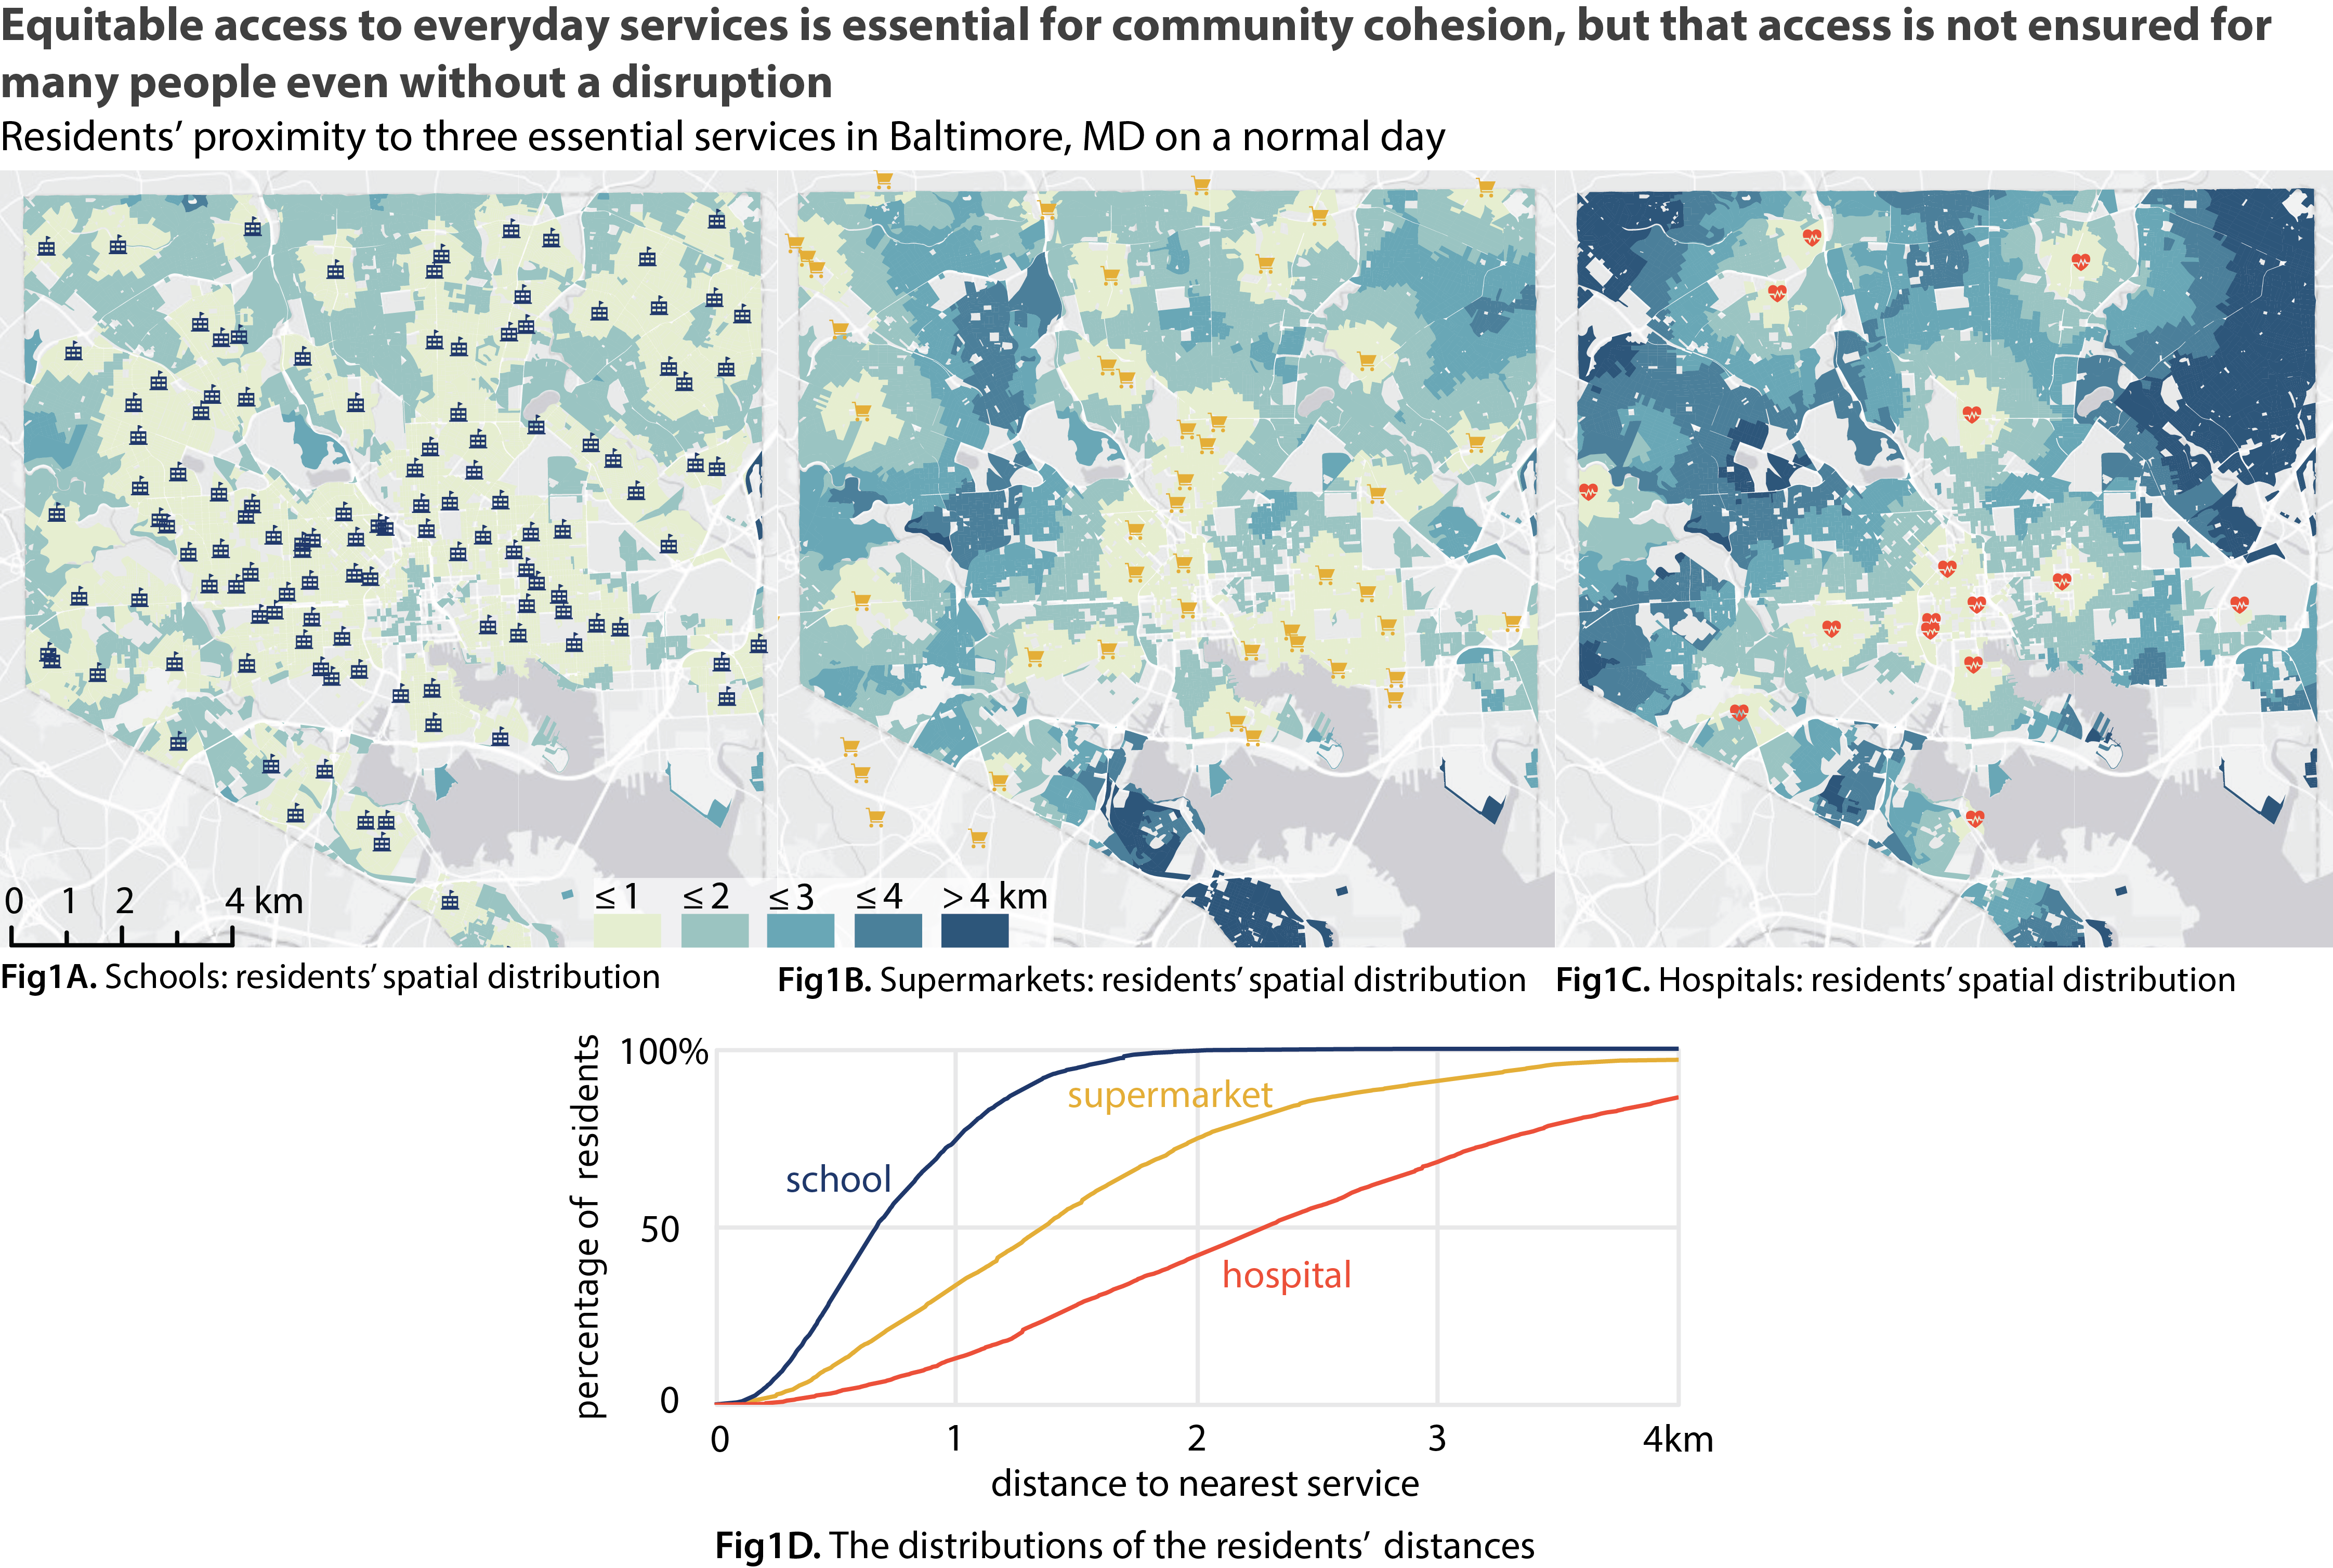
\includegraphics[width=\linewidth]{report/fig/fig_bal.png}
    \caption{Equitable and acceptable access to services is essential for a communities viability and cohesion. These maps of Baltimore, MD, show the distance to the nearest (a) public primary school, (b) supermarket, (c) hospital. Fig. (d) shows the percentage of residents who live within $x$ kilometers of their nearest service.
    }
    \label{fig:bal_services}
\end{figure*}

Key to fostering community resilience is social capital (the ability to use relationships to meet one's needs and access resources), social cohesion, networks, and a sense of place \cite{Dempsey2011-og,Berkes2013-jr, Cutter2008-placeBasedModel}.
The built environment, e.g., active street fronts, mixed-use development, and destinations, plays a major role in encouraging these values in a neighborhood \cite{Bramley2009-ol, Talen1999-sx,Frumkin2004-yi}.
Providing equitable access to everyday services underpins a sustainable community \cite{Dempsey2011-og}, and in-turn is essential for the community's ability to prepare for and respond to a disaster: their resilience.

Therefore, we propose that community resilience be thought of in terms of a community's equitable access to essentials (EAE).
One way to operationalize this framing of resilience, and the approach we devise and illustrate, is to measure the distance of residents within a community to their nearest operational essential services. 
As facilities shutter and reopen due to some hazard, we can evaluate what percentage of people are affected, how long it takes to recover, and how the experiences differ across different groups of the population. 
This would provide a spatially and temporally explicit approach that both 1) identifies where and who requires attention from emergency responders, and 2) enables interventions to reduce service deserts (e.g., food), both before and after a hazard, reducing inequity and strengthening the communities.

In practice, this may look like Figures \ref{fig:NC_resil_super} or \ref{fig:NC_resil_gas}.
In this illustrative example, which is one of two that we present in detail in Section \ref{sec:illustrative}, we evaluate the access of supermarkets and service stations in Wilmington, North Carolina over the course of 2018's Hurricane Florence.
We introduce this figure to provide a concrete example of how reframing resilience as access to essentials could be done.
The objective is to 1) understand the spatial extent of service disruption so service-poor residents can be identified, 2) evaluate the community's resilience to this hazard. 
Our use of grocery stores and service stations is for demonstration purposes, based on available open-source data.
Fig. \ref{fig:NC_resil_super}(a) presents the city's residential blocks and is colored by the distance to the nearest open supermarket.
Fig. \ref{fig:NC_resil_super}(b) presents the statistical distribution that shows the percentage of residents within $x$ distance of their nearest service.
Fig. \ref{fig:NC_resil_super}(c) is an example of a resilience or recovery curves showing how the distance to nearest service changes over time; these resilience curves include the distribution of residents' access so that inequality can be identified.
As EAE is generalizable to the amenity considered, we also show how it would be applied to service stations in Fig. \ref{fig:NC_resil_gas}

\begin{figure*}
    \centering
    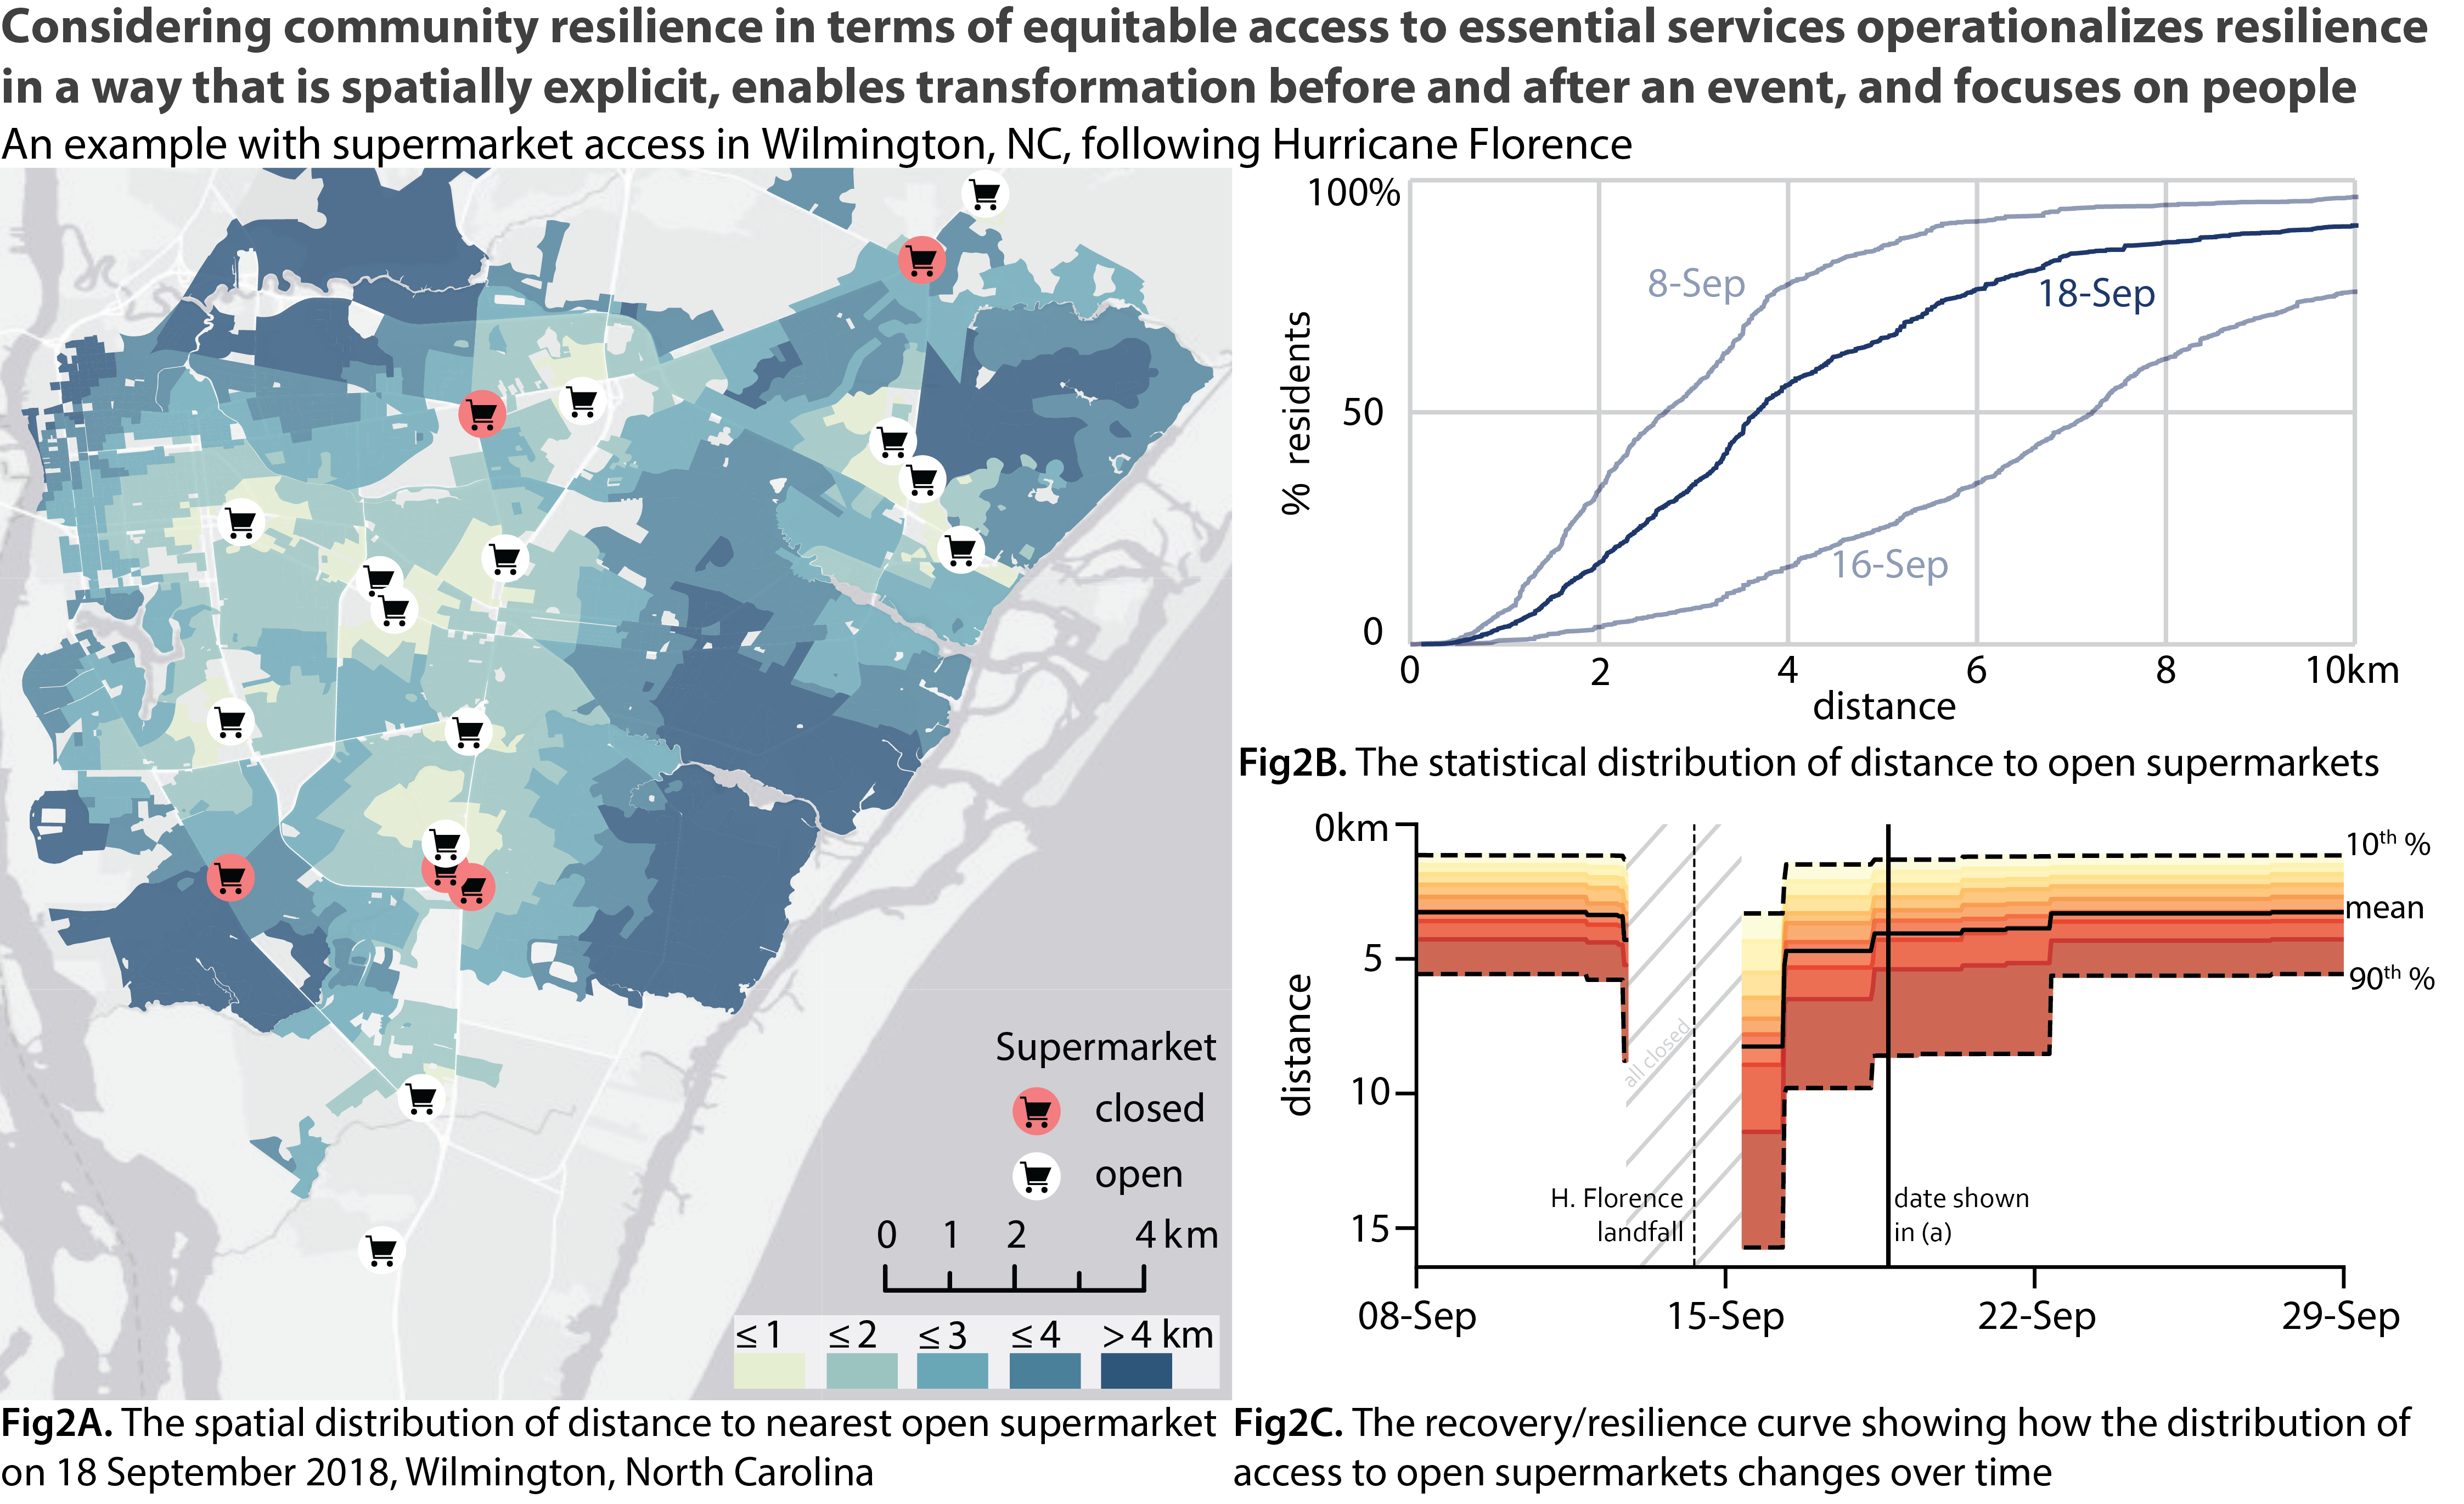
\includegraphics[width=\linewidth]{report/fig/NC_supermarket_resilience.png}
    \caption{An example of the equitable access to essentials approach to resilience using supermarket access in Wilmington, NC and how it was affected due to Hurricane Florence. (a) The map of distance to nearest operational supermarket for census blocks with non-zero populations, (b) the cumulative distribution function showing the percentage of residents who are closer than $x$ to their nearest operational service, and (c) the resilience curve showing how the distribution in access changes over time.
    }
    \label{fig:NC_resil_super}
\end{figure*}
\begin{figure*}
    \centering
    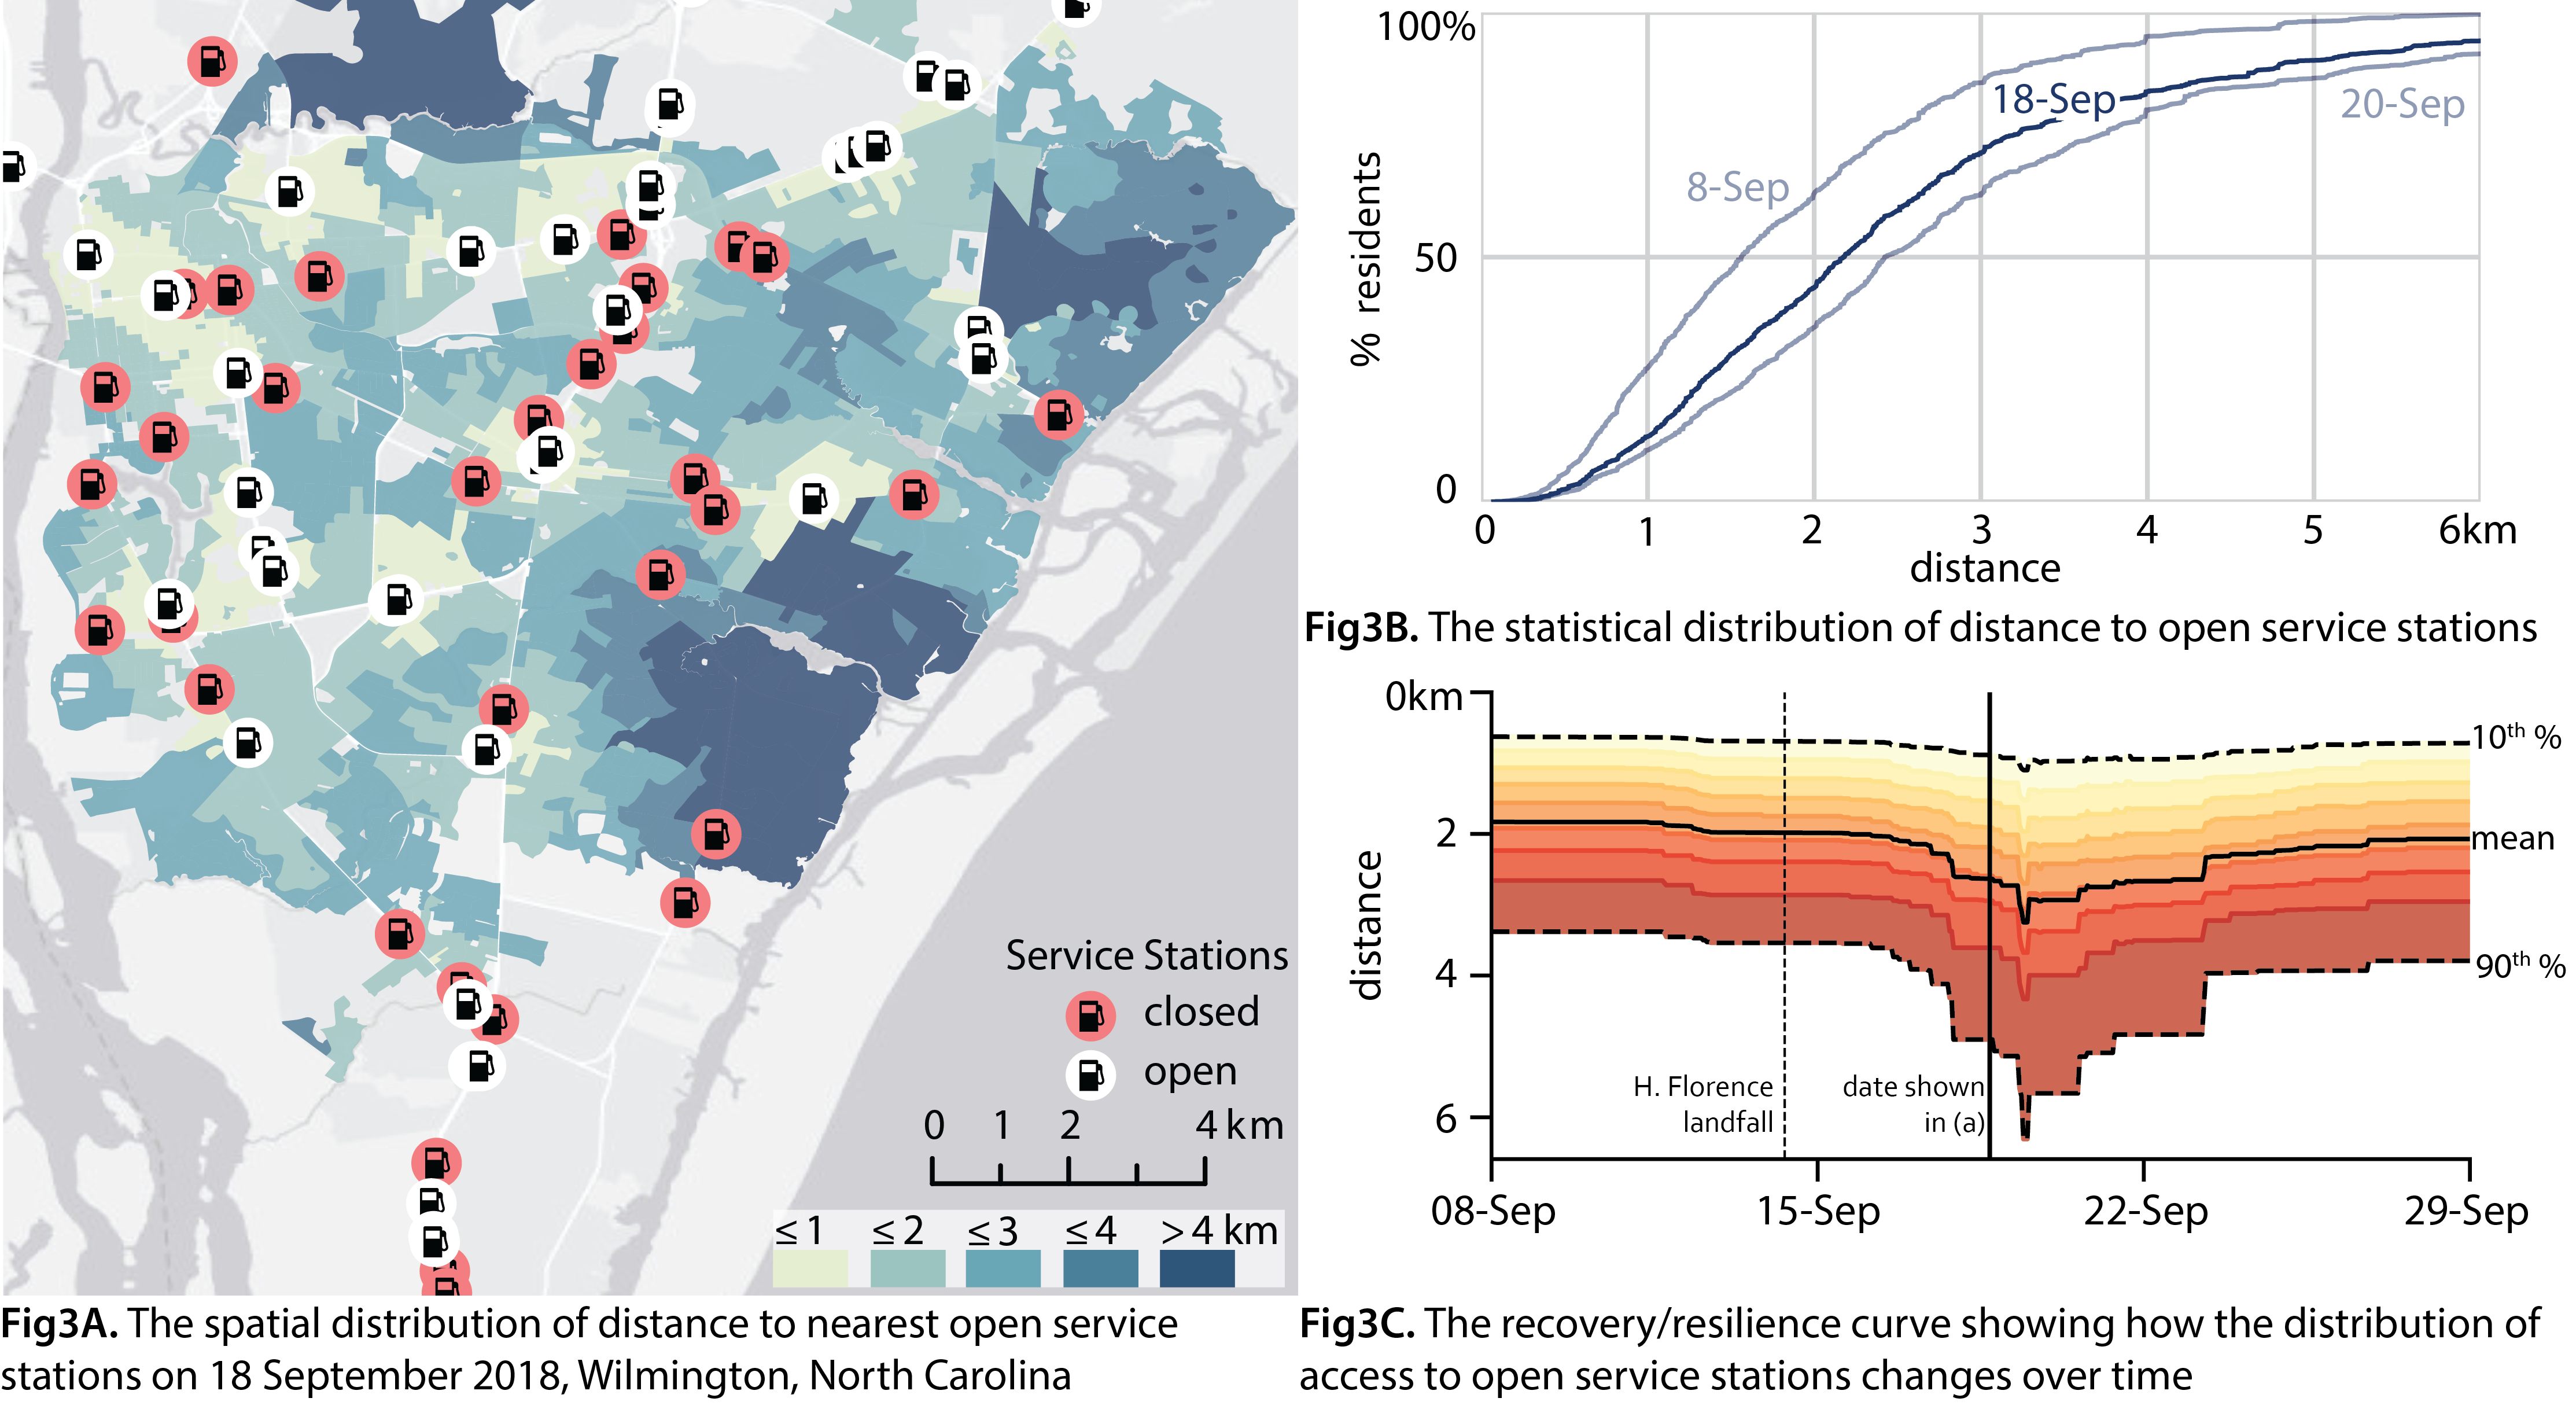
\includegraphics[width=\linewidth]{report/fig/NC_gasstation_resilience.png}
    \caption{Another example of the equitable access to essentials approach to resilience in Wilmington, NC, this time using service stations to demonstrate the generality of the approach.}
    \label{fig:NC_resil_gas}
\end{figure*}

Although we present an example for hurricanes, the EAE approach to resilience is general and is thus applicable for a wide range of hazards. 
For example, before any hazardous event, EAE can be used to address inequality and to identify critical service locations by simulating a set of potential future hazards. 
Following a hazard that damages services or their supporting infrastructure, such as an earthquake or weather-induced event (hurricane, flooding, heat wave), EAE can guide decision making on restoration.
Following any hazard, regardless of the scale of destruction, EAE could support decision-makers on where supplies need to be provided.
In the event of a complete destruction, such as the result of a major wildfire or even sea level rise, EAE can guide new, or green-field, development to ensure it meets the needs of people.

%%%%%%%%%% How does this integrate the existing methods?
This new way of framing community resilience, in terms of equitable access to essential services, is one that can support building community resilience.
This approach can integrate information from both the critical infrastructure and community capacity approaches to resilience.
For example, we could estimate the threat to service-access based on critical infrastructure risk and then evaluate the community need and assess equity using 
the community characteristics and social vulnerability.
Therefore, conceptualizing resilience as equitable access to essentials provides a new direction for resilience implementation that integrates the existing approaches and provides a clear focus on the well-being of the community's residents.

\section{Key aspects and further research}
In proposing the EAE framing of community resilience, we leverage both of the dominant approaches to resilience. 
We also integrate accessibility, spatial planning, and land use research, into the conversation.
In this section, we describe some of the rationale underlying the proposed framing and identify areas for further research and development.

\subsection{Types of essential services}
Every community will have different services they consider essential.
Although lists of local services and facilities to which residents need everyday access exist (e.g., \citeA{Dempsey2011-og}), our approach does not prescribe them.
Instead, we encourage community engagement to identify the important services to reflect the local and cultural needs.
While we focus on services requiring people to go to centralized locations, services that send people from central locations, such as ``Meals on Wheels," can also be included.
The approach's flexibility means that (re)construction focuses on places and services of significance to people \cite{United_Nations_Educational_Scientific_and_Cultural_Organization2018-sf}.

\subsection{Accessibility}
Defining and measuring access is an active field of research that has been approached from perspectives including planning, facility location, public health, medicine, and ecosystem services \cite{Penchansky1981-qh,Saurman2016-gj,Talen2003-dc, Talen1998-mk, Logan2017-fr, noel2019-pypi}.
Access generally includes the dimensions of proximity, availability, acceptability, affordability, adequacy, and awareness \cite{Saurman2016-gj, Penchansky1981-qh}. 
We demonstrate the EAE approach to community resilience using proximity in our illustrative example.
Proximity is a necessary component for access to services and provides insight into the resilience of a community. 
Nevertheless, the EAE framing of resilience can incorporate other measures of access, requiring additional work that draws from and advances the accessibility literature.

In practice, this could be implemented by using a metric that defines acceptable access.
This would specify a minimum level suitable for human well-being \cite{Doorn2018-fx}.
In the future it may enable the proximity, cost, capacity, and other dimensions of accessibility to vary based on the characteristics and vulnerabilities of the community to consider social justice (for example, proximity may vary based on car-ownership).
This standard should be normatively indexed, i.e., any standard of access should be relative to the community and may change over time \cite{Constas2014-ui}.
Fig. \ref{fig:threshold} demonstrates the use of a metric, in this case specified as a distance threshold for proximity.
The percentage of the residents with acceptable access is shown by the cumulative distribution functions (the process is shown in Fig. \ref{figS:cdf_to_res}). 
The threshold must be place-based and service-specific and determined through community engagement \cite{Pantelic1991-qu, United_Nations_Educational_Scientific_and_Cultural_Organization2018-sf}.
This means we can specify a minimum acceptable standard of accessibility for each of the services and determine the portion of the community with acceptable access.

However, a major benefit of using a continuous measure of access, such as proximity, is the ability to assess the distribution of access across the population. 
There is a very real risk when using thresholds that the residents with extremely poor access, who are often among the most vulnerable, are overlooked because they are aggregated by a binary metric \cite{Logan2017-fr}. 
This is especially important given that poverty often lies at the root of disaster vulnerability, so true resilience approaches must help correct this \cite{Pantelic1991-qu}.
Scholars and practitioners must be cognizant of this risk when defining the metrics they use so they do not inadvertently discriminate. 

%%%%%%%%%% Equity and targeting vulnerability
\subsection{Equality and equity}

\begin{figure*}
    \centering
    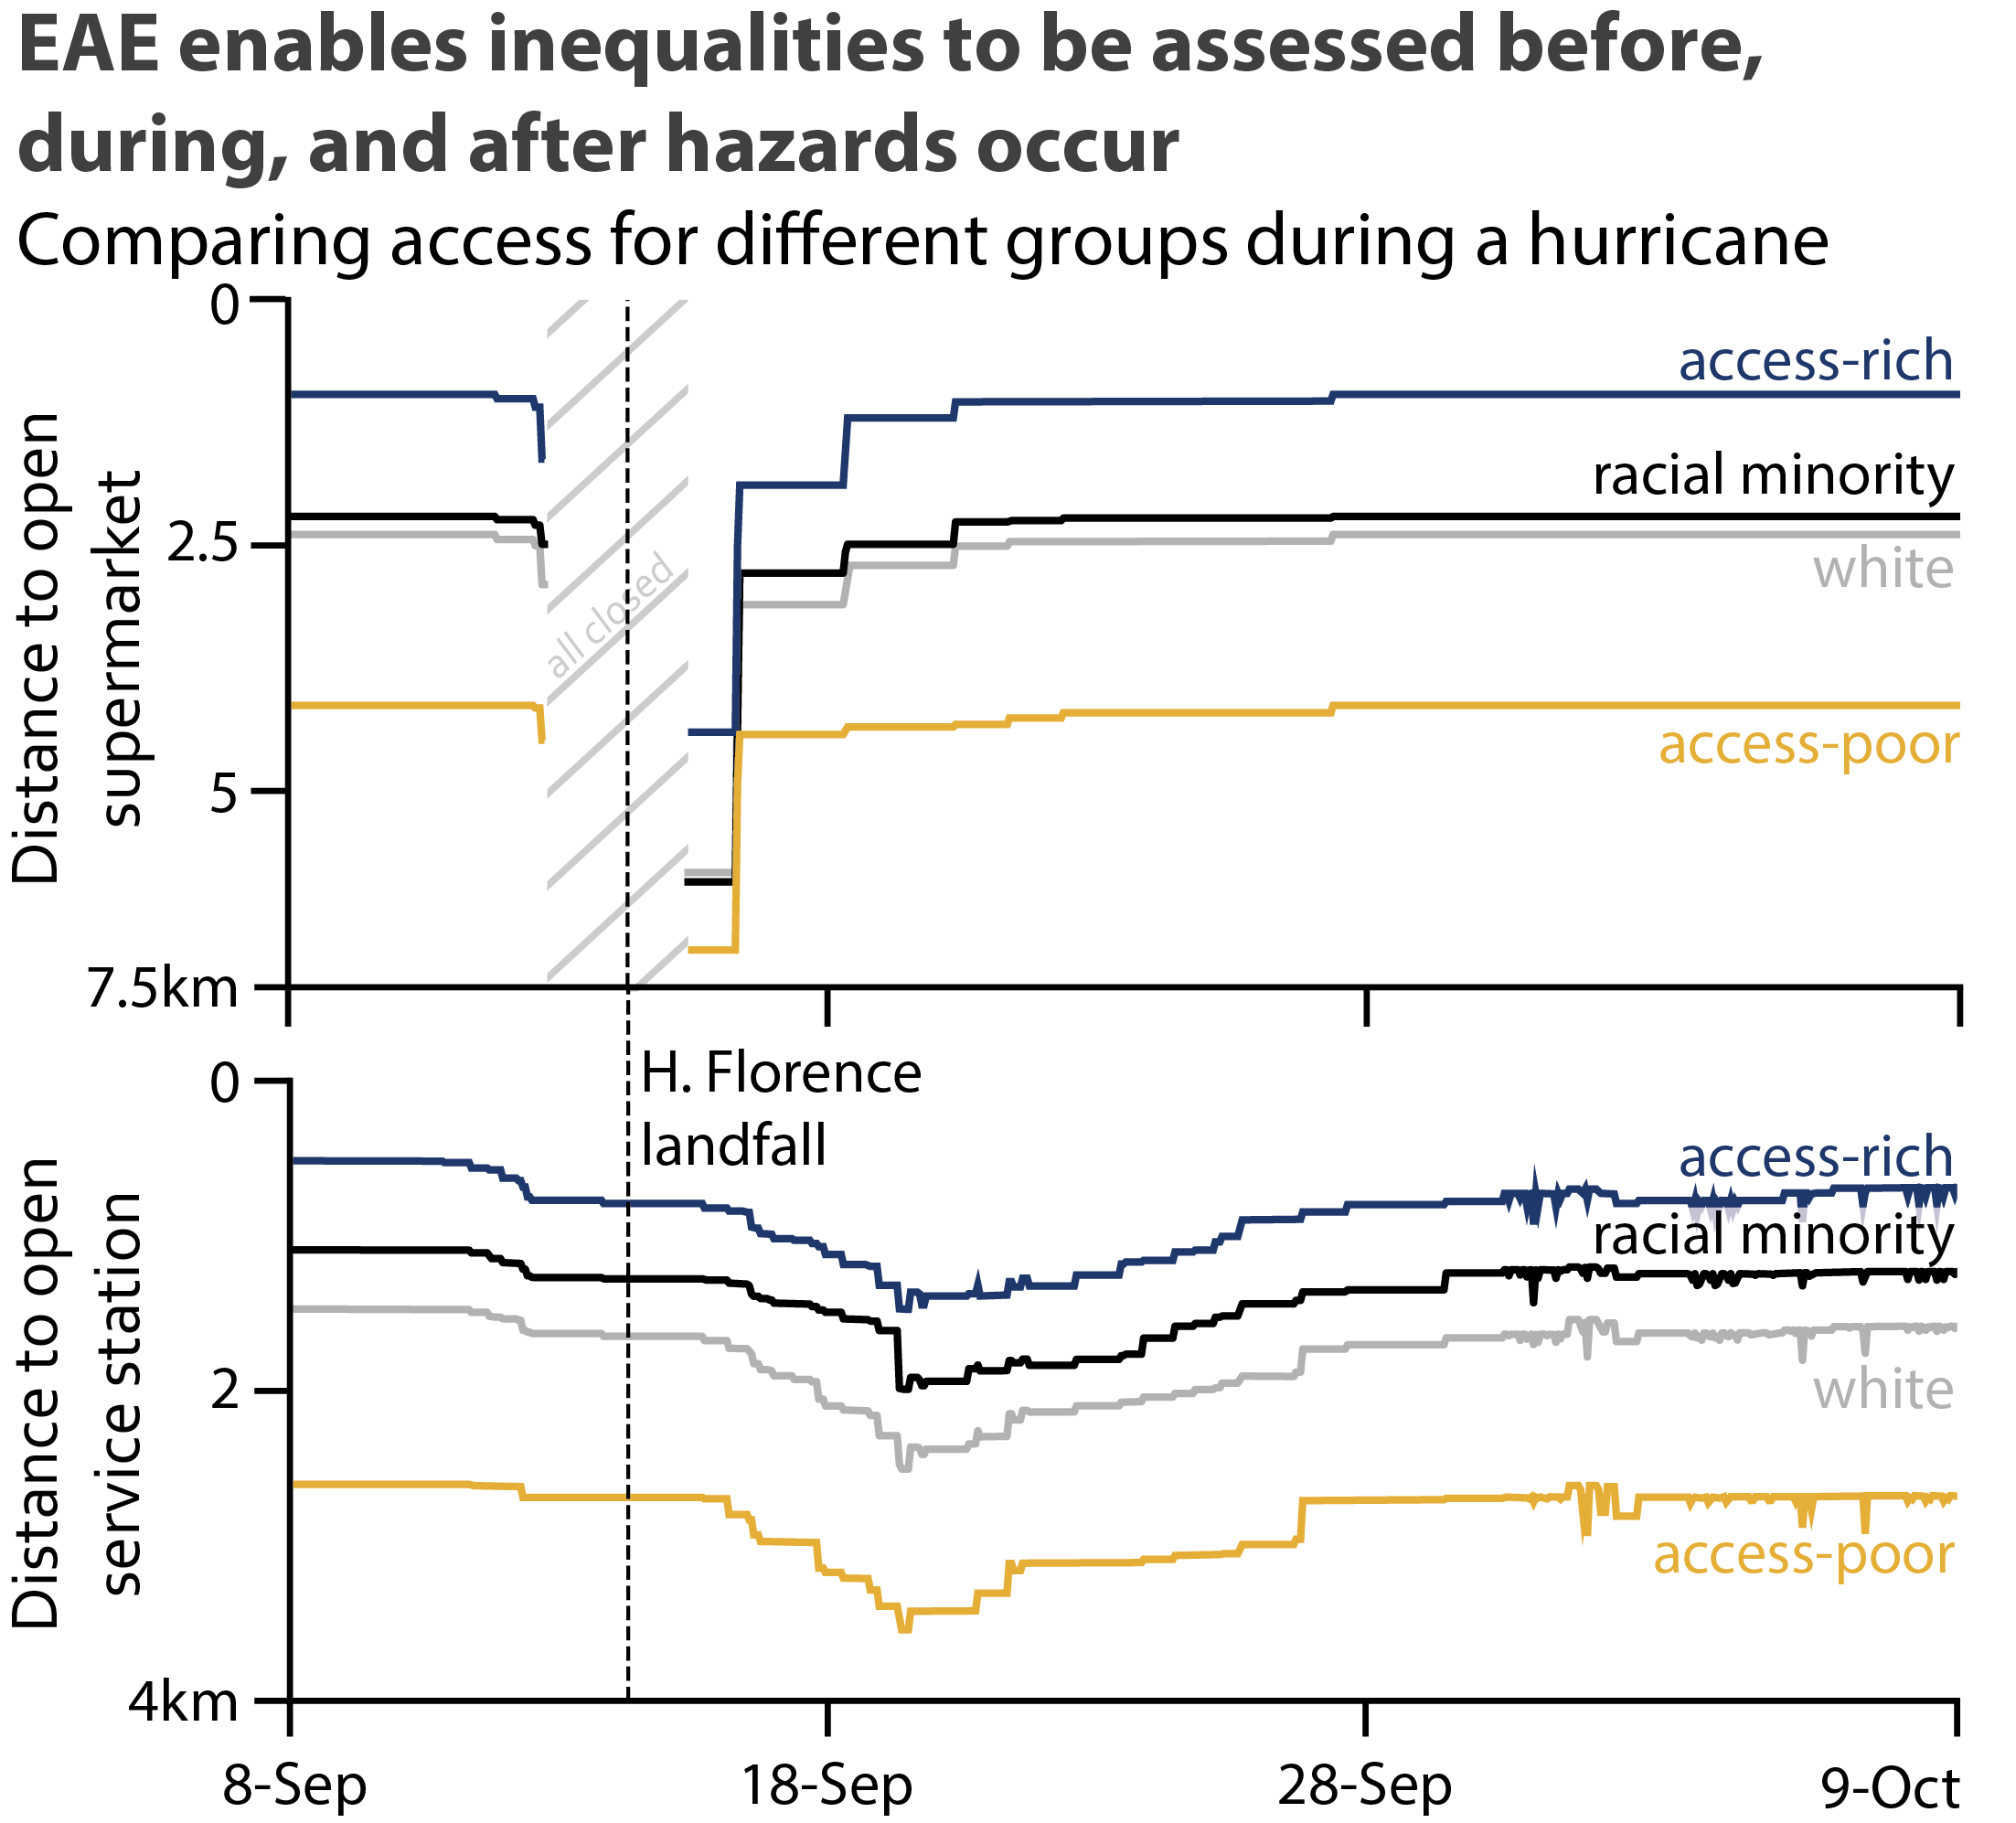
\includegraphics[width=0.5\linewidth]{report/fig/equality_NC.png}
    \caption{Comparing how access to essentials varies between demographic groups and initially access-rich/poor residents (the top and bottom 20\% of residents). This could also be done based on indicators of social vulnerability or community capacity.}
    \label{fig:equality}
\end{figure*}

A major consideration for resilience measurement and implementation is the effect on equality and equity \cite{Matin2018-pg}.
Inequalities may be present before the occurrence of a hazard and are often exacerbated after an event \cite{Gardoni2018-xu}.
An EAE approach to resilience can include consideration of socio-economic characteristics and evaluate the accessibility of services across demographic groups (Fig. \ref{fig:equality} is a demonstration based on race and service-wealth) \cite{Williams_undated-sy}.
This enables needs-based assessments and the integration of indicators of social vulnerability and community capacity.
Potential interventions could subsequently be assessed based on the effect on different groups within the community.

%%%%%%%%%%%% Transformation
\subsection{Promoting transformation}
Inequity and inequality can inadvertently also be institutionalized by resilience approaches that prioritize ``bouncing back", and quantify resilience using a ``change-in functionality" \cite{Normandin2019-hp, I_Sudmeier-Rieux2014-lc, MacKinnon2013-nx}.
Claims such as ``residents have grown used to'' these abysmal conditions, fail to value the importance of equity and community sustainability for resilience to future events \cite{Dempsey2011-og, Pantelic1991-qu}.
They fail because they do not promote transformation and mitigation that encourages communities to ``bound forward.''

The EAE approach promotes transformation of communities to enhance equity, both before and after a disruption, in two ways.
First, unlike the critical infrastructure approach, which predominantly focuses on the state of infrastructure damage \cite{Cutter2010-vg}, EAE assesses the value residents derive from the system. 
This distinction is important because restoring functionality is not analogous to returning to the previous state e.g., the services can be rebuilt in more desirable spatial configurations.
Second, by assessing actual distance, rather than the difference at any point in time with the initial state (``change-in"), EAE enables identificatoin of the service-poor residents. 
For example, in Fig. \ref{fig:equality}, the largest change in access is experienced by the service-rich residents.
If decisions were made on the basis of this differential, then interventions would be targeted to improve the resilience of service-rich residents and further exacerbate inequalities.
Instead, decision-makers should be aware of pre- and post-hazard service deserts. 
This should mean that both mitigation and reconstruction target and improve the standard of living for all residents \cite{Pantelic1991-qu}, which is essential for building sustainable communities that are enabled to enhance their adaptive capacity and future resilience \cite{Saunders2015-uz}.

\subsection{Spatially explicit}
Place-specific information is important to guide decision-makers when building community resilience \cite{Frazier2013-ct}.
The majority of existing approaches to resilience are spatially coarse.
Most do not explicitly require information about a community's layout nor do they support urban planners in spatial planning. 
Developments have improved this and include spatial dependencies \cite{Frazier2013-ct}, but still rely on indicators that are independent of the critical infrastructure state.
An output of an EAE approach is the access map, which serves as an integral decision-support tool.
Examining the EAE maps allows decision-makers to understand the distribution of damage, vulnerable people, and services and act accordingly.

More generally, integrating land-use planning with resilience quantification is essential because spatial planning is among the most effective tools for reducing exposure and sensitivity to extreme events \cite{Brunetta2019-ki, Campbell2006-in, Hurlimann2012-uj, Berke2015-nv} (see \citeA{Anderson2018-hr} for climate related examples). 
Surprisingly, there has been little attempt to integrate climate protection and spatial planning in practice \cite{Barnes2017-xf}.
Taking an EAE approach to resilience brings spatial planning to the forefront of resilience quantification by clearly linking it with urban changes and social sustainability.
Incorporating EAE into planning can identify service-deserts and key facilities that many people depend on.
This can guide urban planners to strengthen existing facilities or incentivize the development of additional ones.
Additionally, it can be used to guide both green and brown field development to ensure that people's access to essential services is provided equitably.
In this way, EAE links policy discussion regarding accessibility and equity with resilience and hazard planning.
This supports rethinking how our cities are designed, planned, managed, and lived in, in the pursuit of community and urban resilience \cite{Caldarice2019-tv}. 

\subsection{Application throughout the hazard cycle}
\begin{figure}
    \centering
    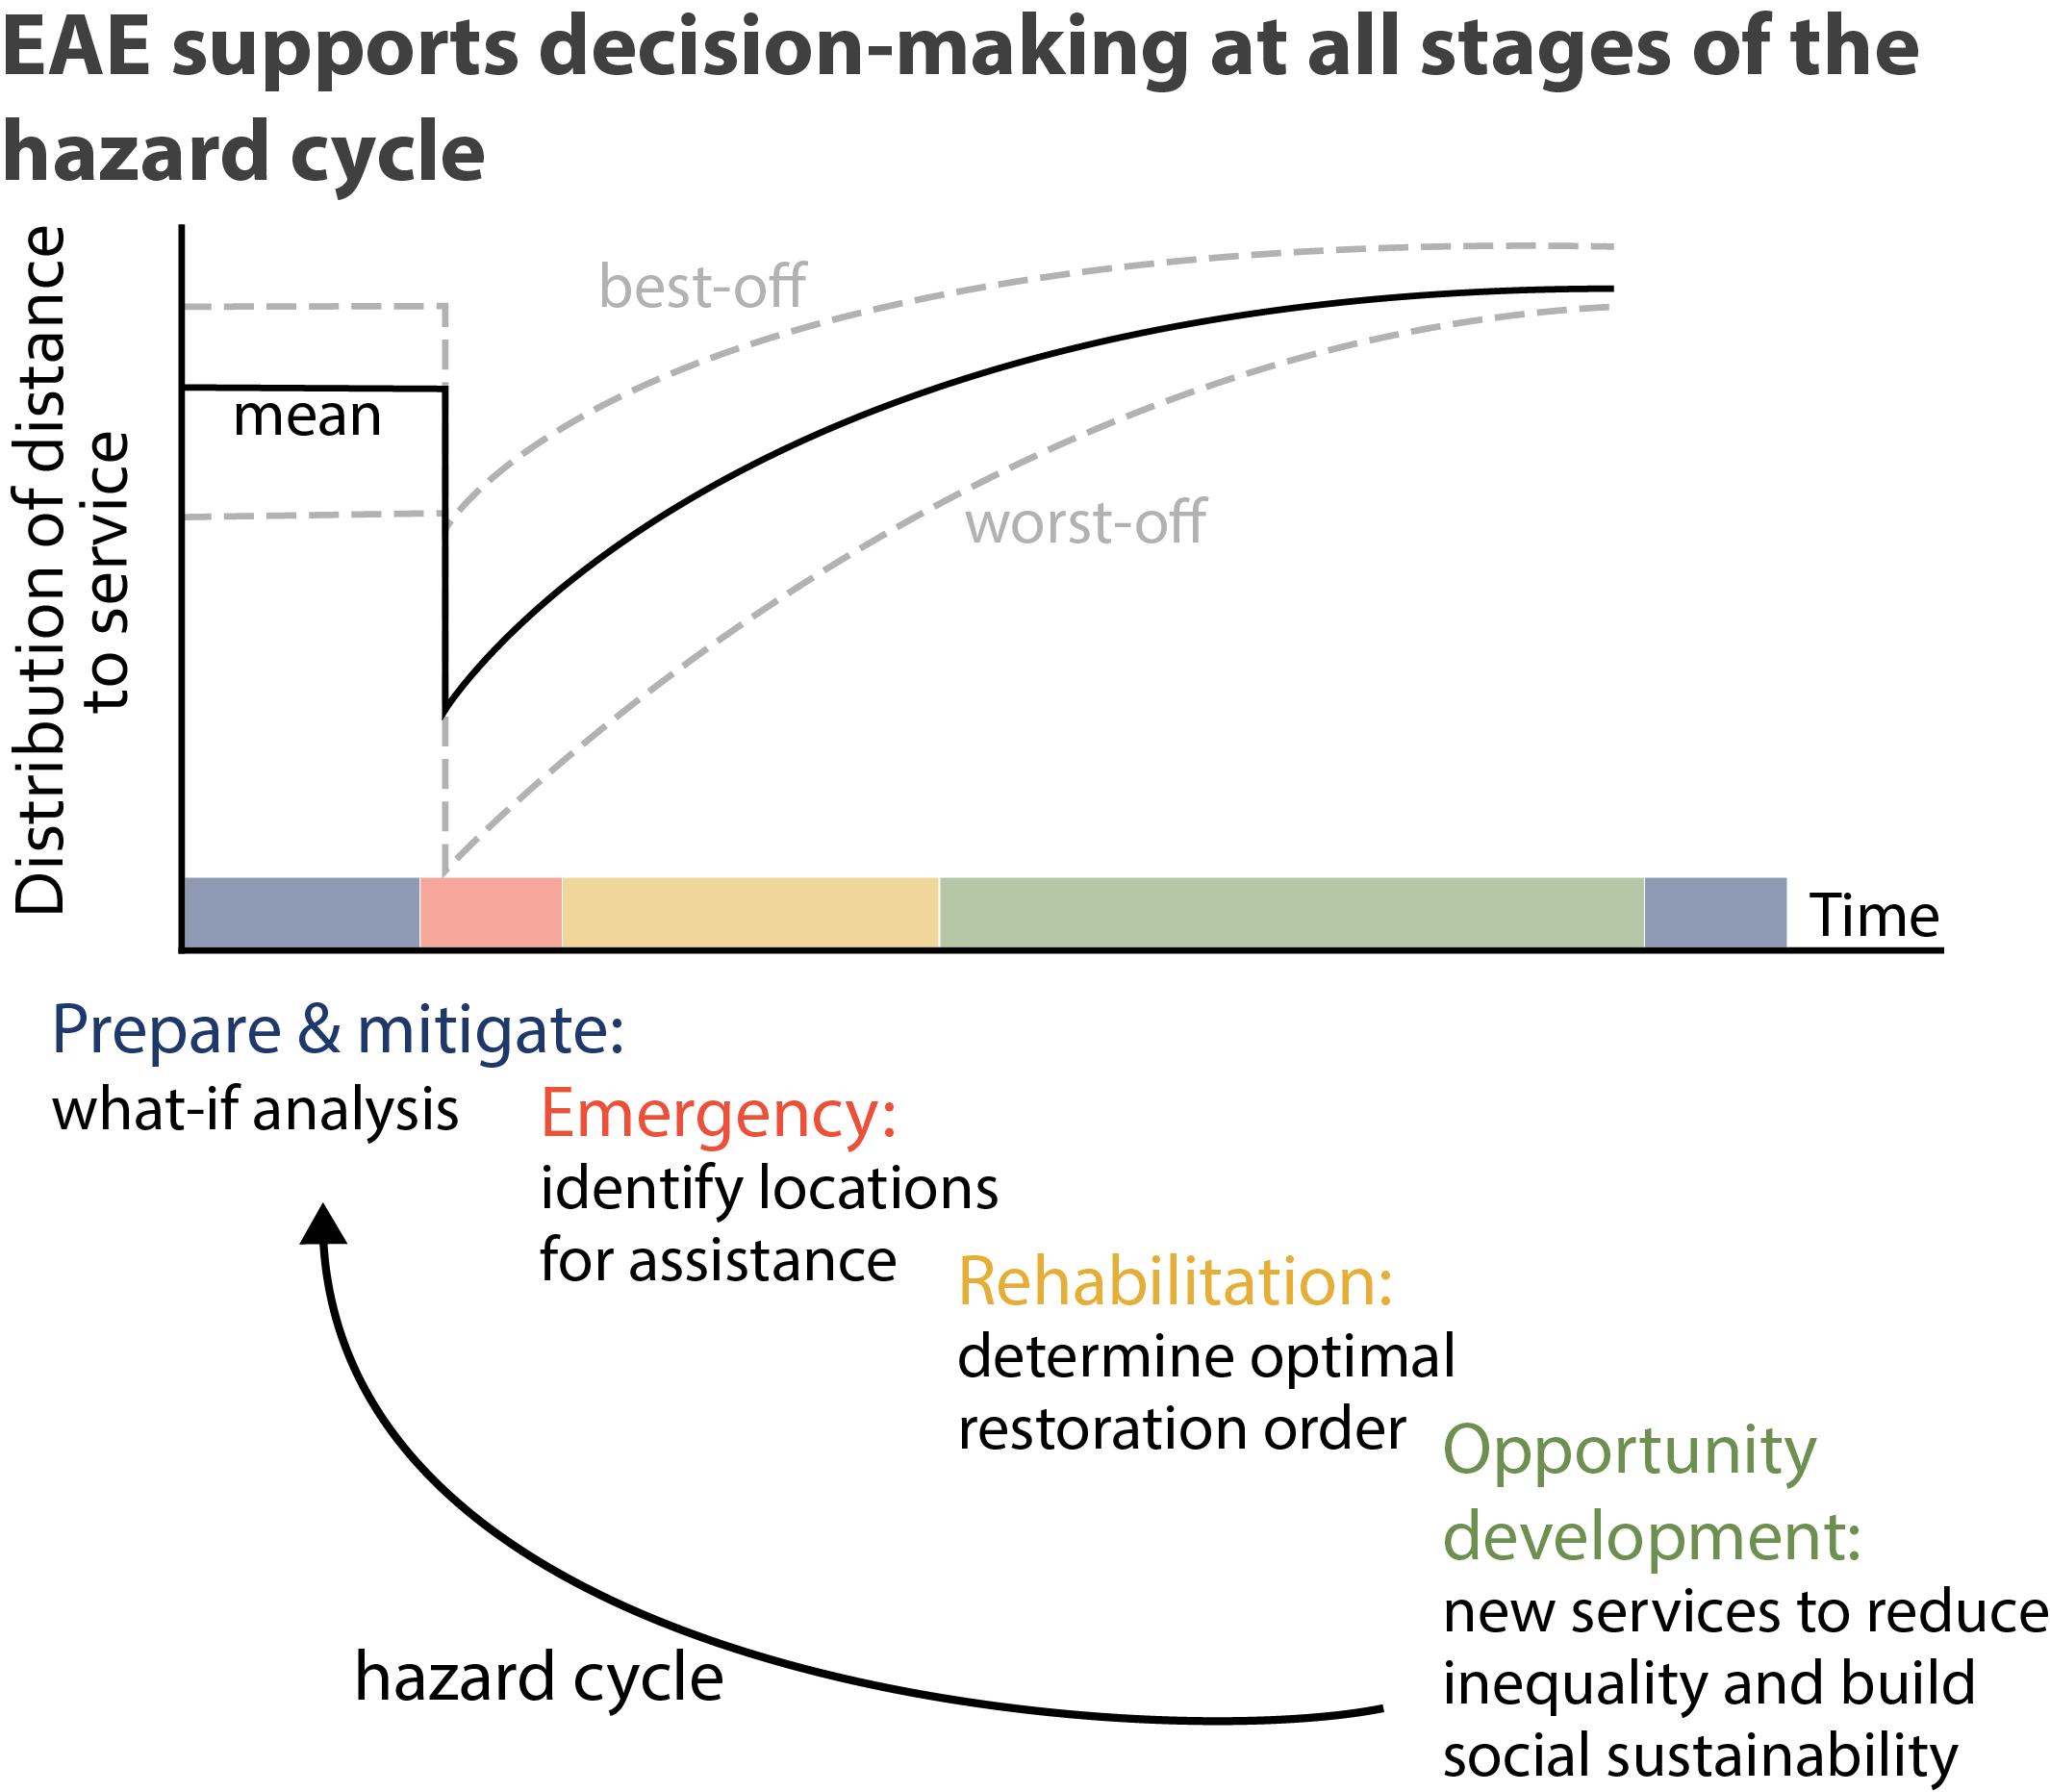
\includegraphics[width=0.5\linewidth]{report/fig/hazard_cycle.png}
    \caption{This resilience function (aka recovery curve) shows how the access, and its distribution, may change before, during, and after a hazard. The hazard cycle shows how the EAE resilience approach could be utilized by decision-makers from mitigation to recovery.}
    \label{fig:haz_cycle}
\end{figure}
Resilience as EAE can inform decision making throughout the hazard management cycle. 
The cycle (Fig. \ref{fig:haz_cycle}) involves preparing for and mitigating potential hazards; emergency response; and recovery, including the immediate rehabilitation and longer term (re)construction: opportunity development.

Implementing this approach in the field will require real-time information about the functioning of services.
For example, local networks or reporting systems could be implemented.
This, coupled with improvements in proximity analysis \cite{Logan2017-fr, noel2019-pypi}, mean that essential service access can be evaluated before, during, and after a hazard strikes.
This can be used to guide emergency response as well as short-term and long-term recovery and development. 

\subsubsection{Mitigation and preparedness}
Before any hazard occurs, existing inequities to service-deserts should be addressed.
This will enhance community cohesion and social capital (Section \ref{sec:eae}, \citeA{Dempsey2011-og}) and provide residents with opportunities \cite{Cutter2010-vg}.
Additionally, ``what-if" simulation can determine which facilities are critical in servicing the community. 
This type of analysis can be used to build redundancy or robustness into the system \cite{Wardekker2010-hw}.

\subsubsection{Emergency response}
During and immediately following a disruption, an EAE-based approach could enable responders to identify impacted areas and allocate resources appropriately. 
To leverage this tool, appropriate data collection systems are needed. 
This could be simply scraping websites such as Twitter or GasBuddy, or, ideally, could be a crowd-sourced setup where facilities or the public report damage or closures, similar to the ``call 311'' system used by a number of USA cities to report non-emergency problems.
Such data would allow the service accessibility map to be updated in real-time and would support targeting supplies like food and health care to places in need. 
Based on population characteristics, vulnerabilities and needs could be considered so that situations such as the ignoring of vulnerable residents in the Rockaways, NY, following Hurricane Sandy \cite{Subaiya2014-qx}, do not reoccur. 

\subsubsection{Rehabilitation} 
During this phase, short-term and basic essential services are restored \cite{Resendiz-Vazquez2019-ol}. 
Facility reopening can be coordinated and optimized to maximize accessibility.
Where relocation is required, using an EAE approach would avoid the situation in which residents of L'Aquila, Italy, found themselves following the 2009 earthquake \cite{Contreras2017-yq}.
People were discontent and left the relocation settlements because of a lack of urban amenities including churches, schools, pharmacies, etc. 
Instead, with an EAE tool, sites can be evaluated and planned so that there is equitable access to everyday amenities.

\subsubsection{Opportunity development}
This latter phase of recovery is referred to as ``opportunity development'' rather than reconstruction (returning to the previous state) \cite{Resendiz-Vazquez2019-ol,Pantelic1991-qu}. 
We should build back better \cite{Resendiz-Vazquez2019-ol} by not only enhancing protection against future hazards \cite{Platt2019-lx}, but by improving equity and residents’ quality of life \cite{Pantelic1991-qu}. 
In this phase, different policy mechanisms must be leveraged to encourage desired amenities such as grocery stores to establish in certain locations. 
For example, comprehensive plans can be used to set minimum numbers for food retailers, zoning mechanisms can simplify the regulatory process, and subsidies or other incentives can recruit retailers to in-need areas \cite{Raja2010-cm, Raja2008-wx}. 

\section{A methodology for implementation}
For a specified region, assessing the resilience as equitable access to essentials would involve: 
\begin{enumerate}[topsep=1pt,itemsep=0em,partopsep=1ex,parsep=1ex]
    % \itemsep0em
    \item Engaging the community 
    \begin{enumerate}[topsep=0pt,itemsep=-2pt,partopsep=1ex,parsep=1ex]
        % \itemsep0em
        \item Establish which services are essential, and how needs differ throughout the community
    \end{enumerate}
    \item Measuring accessibility
    \begin{enumerate}[topsep=0pt,itemsep=-2pt,partopsep=1ex,parsep=1ex]
        % \itemsep0em
        \item For each of the essential services, identify the locations of service provision facilities within the region
        \item From each block within the region, determine the network distance to all facilities
        \item For each block, determine the distance to the nearest operational facility
        \item Map the distances to nearest service (Fig. \ref{fig:NC_resil_super}a)
        \item Plot the distribution of nearest distances (Fig. \ref{fig:NC_resil_super}b)
    \end{enumerate}
    \item Monitoring the impacts from a hazard
    \begin{enumerate}[topsep=0pt,itemsep=-2pt,partopsep=1ex,parsep=1ex]
        % \itemsep0em
        \item Update the distance to nearest operational services as facilities open and close
        \item Construct the resilience curve showing how residents' access changes over time (Figures \ref{fig:NC_resil_super}c, \ref{figS:cdf_to_res})
    \end{enumerate}
    \item Evaluating equality and equity (Fig. \ref{fig:equality})
    \begin{enumerate}[topsep=0pt,itemsep=-2pt,partopsep=1ex,parsep=1ex]
        % \itemsep0em
        \item Differentiate residents based on demographics or vulnerability scores
        \item Compare how the access for these various groups changes over time
        \item Identify vulnerable areas to which to provide additional services and improve equity.
    \end{enumerate}
    \item Intervening to build resilience (Fig. \ref{fig:haz_cycle})
\end{enumerate}

We demonstrate steps 2-4 in the following illustrative example. Code for this analysis is available at \url{https://github.com/tommlogan/access_to_essentials}. 

\section{Illustrative examples using open-source data}
\label{sec:illustrative}

\subsection{Overview and scope}
We now present two illustrative examples focused on Wilmington, North Carolina, and Panama City, Florida.
In late 2018 they were struck by Hurricanes Florence and Michael respectively. 
The examples demonstrate how the access to two services (grocery stores and service stations) change due to the hurricanes. 
Specifically, we seek to 1) understand the spatial extent of service disruption so service-poor residents can be identified, 2) assess the resilience of the community to these hazards. 
Note that our use of grocery stores and service stations is for demonstration purposes; in practice, determining which services are essential and what distance is acceptable requires community engagement and typically many more services would be included. 

Wilmington, NC is located on the southeastern North Carolina coast.
It has a population of approximately 120,000 people. 
Hurricane Florence made landfall slightly east of Wilmington in the early hours of September 14, 2018, as a Category 1 hurricane. 
Due to the hurricane's slow movement, it resulted in heavy rainfall beginning September 13, and coupled with strong storm surge, this resulted in heavy flooding. 

By contrast, Panama City, FL, has approximately 37,000 residents and is located along the Emerald Coast of the Florida Panhandle. 
Hurricane Michael made landfall 40km Southeast of Panama City as a Category 4 hurricane on October 10. 
While Florence was notable for its rainfall, Michael caused catastrophic damage due to extreme winds (the strongest in the USA since 1992 with 208 km/h winds) and storm surge. 

\subsection{Inputs}
For this illustrative example we present the access to grocery stores and service stations before and following the hurricanes. 
Service locations were determined using GasBuddy\footnote{https://tracker.gasbuddy.com} and supermarkets were identified manually using Google Maps.
Access to these services was calculated at the US census block (neighborhood block) level and shapefiles and demographic data was sourced from IPUMS \cite{Manson2018-ug}. 
The Open Street Map street network was downloaded from Geofabrik\footnote{http://download.geofabrik.de/}. 
The distance from each block to all services was calculated using the Open Source Routing Machine using the approach described in \citeA{Logan2017-fr}. 
Facility closure was recorded from GasBuddy, Twitter, and the supermarket websites.

\subsection{Results}
Figures \ref{fig:NC_resil_super}, \ref{fig:NC_resil_gas}, \ref{fig:FL_resil_super}, \& \ref{fig:FL_resil_gas} show access in Wilmington and Panama City following the hurricanes. 
The maps can be used to identify service-deserts, and the recovery functions show how quickly the cities restore access and how acceptable that access is.

As an example, there appears to be a food-desert in western Wilmington \ref{fig:NC_resil_super}a, so these residents may require emergency food supplies even after the other stores reopen.
Note that due to data availability, the supermarket results do not include all food outlets as we only obtained information for stores that were reporting their opening times.
Although these results do not comprehensively present food-deserts, they provide a demonstration of using this approach.
These maps could be varied to highlight sectors of the community with high social vulnerability, or, for example, a higher proportion of aged residents, so that emergency response can target need.

Recovery times and access quality are shown in Figures \ref{fig:NC_resil_super}c, \ref{fig:NC_resil_gas}c, \ref{fig:FL_resil_super}c, \ref{fig:FL_resil_gas}c, and \ref{fig:threshold}. 
Supermarkets appear to reopen faster than service stations, likely due to resources provided by their parent companies.
In Wilmington, this was a matter of days.
Access to service stations in Wilmington was still deteriorating by the time supermarket access was almost restored (Figures \ref{fig:NC_resil_gas}c \& \ref{fig:threshold}).
This is likely due to failures in the supply chains.
However, inventory information for supermarkets was unavailable to us.

In Panama City, the recovery took significantly longer for both supermarkets and service stations (Fig. \ref{fig:threshold}).
However, this comparison does not reflect differences between the cities' resilience, because the hurricanes were different. 
Nevertheless, it is clear that Panama City suffered more and for longer.

In both cities, access to supermarkets is less than desirable (Fig. \ref{fig:threshold}).
Even before the hurricanes, only 30\% of residents in Wilmington live within 1 mile (1600 meters), which is further than the majority of distance thresholds considered acceptable (e.g., \citeA{Talen2003-dc}).
This is worse in Panama City, but the results are skewed due to our omission of some food stores that would be included in practice.
Regardless, this shows that there are likely service-deserts existing within the cities that could be mitigated prior to a hazard.

\begin{figure*}
    \centering
    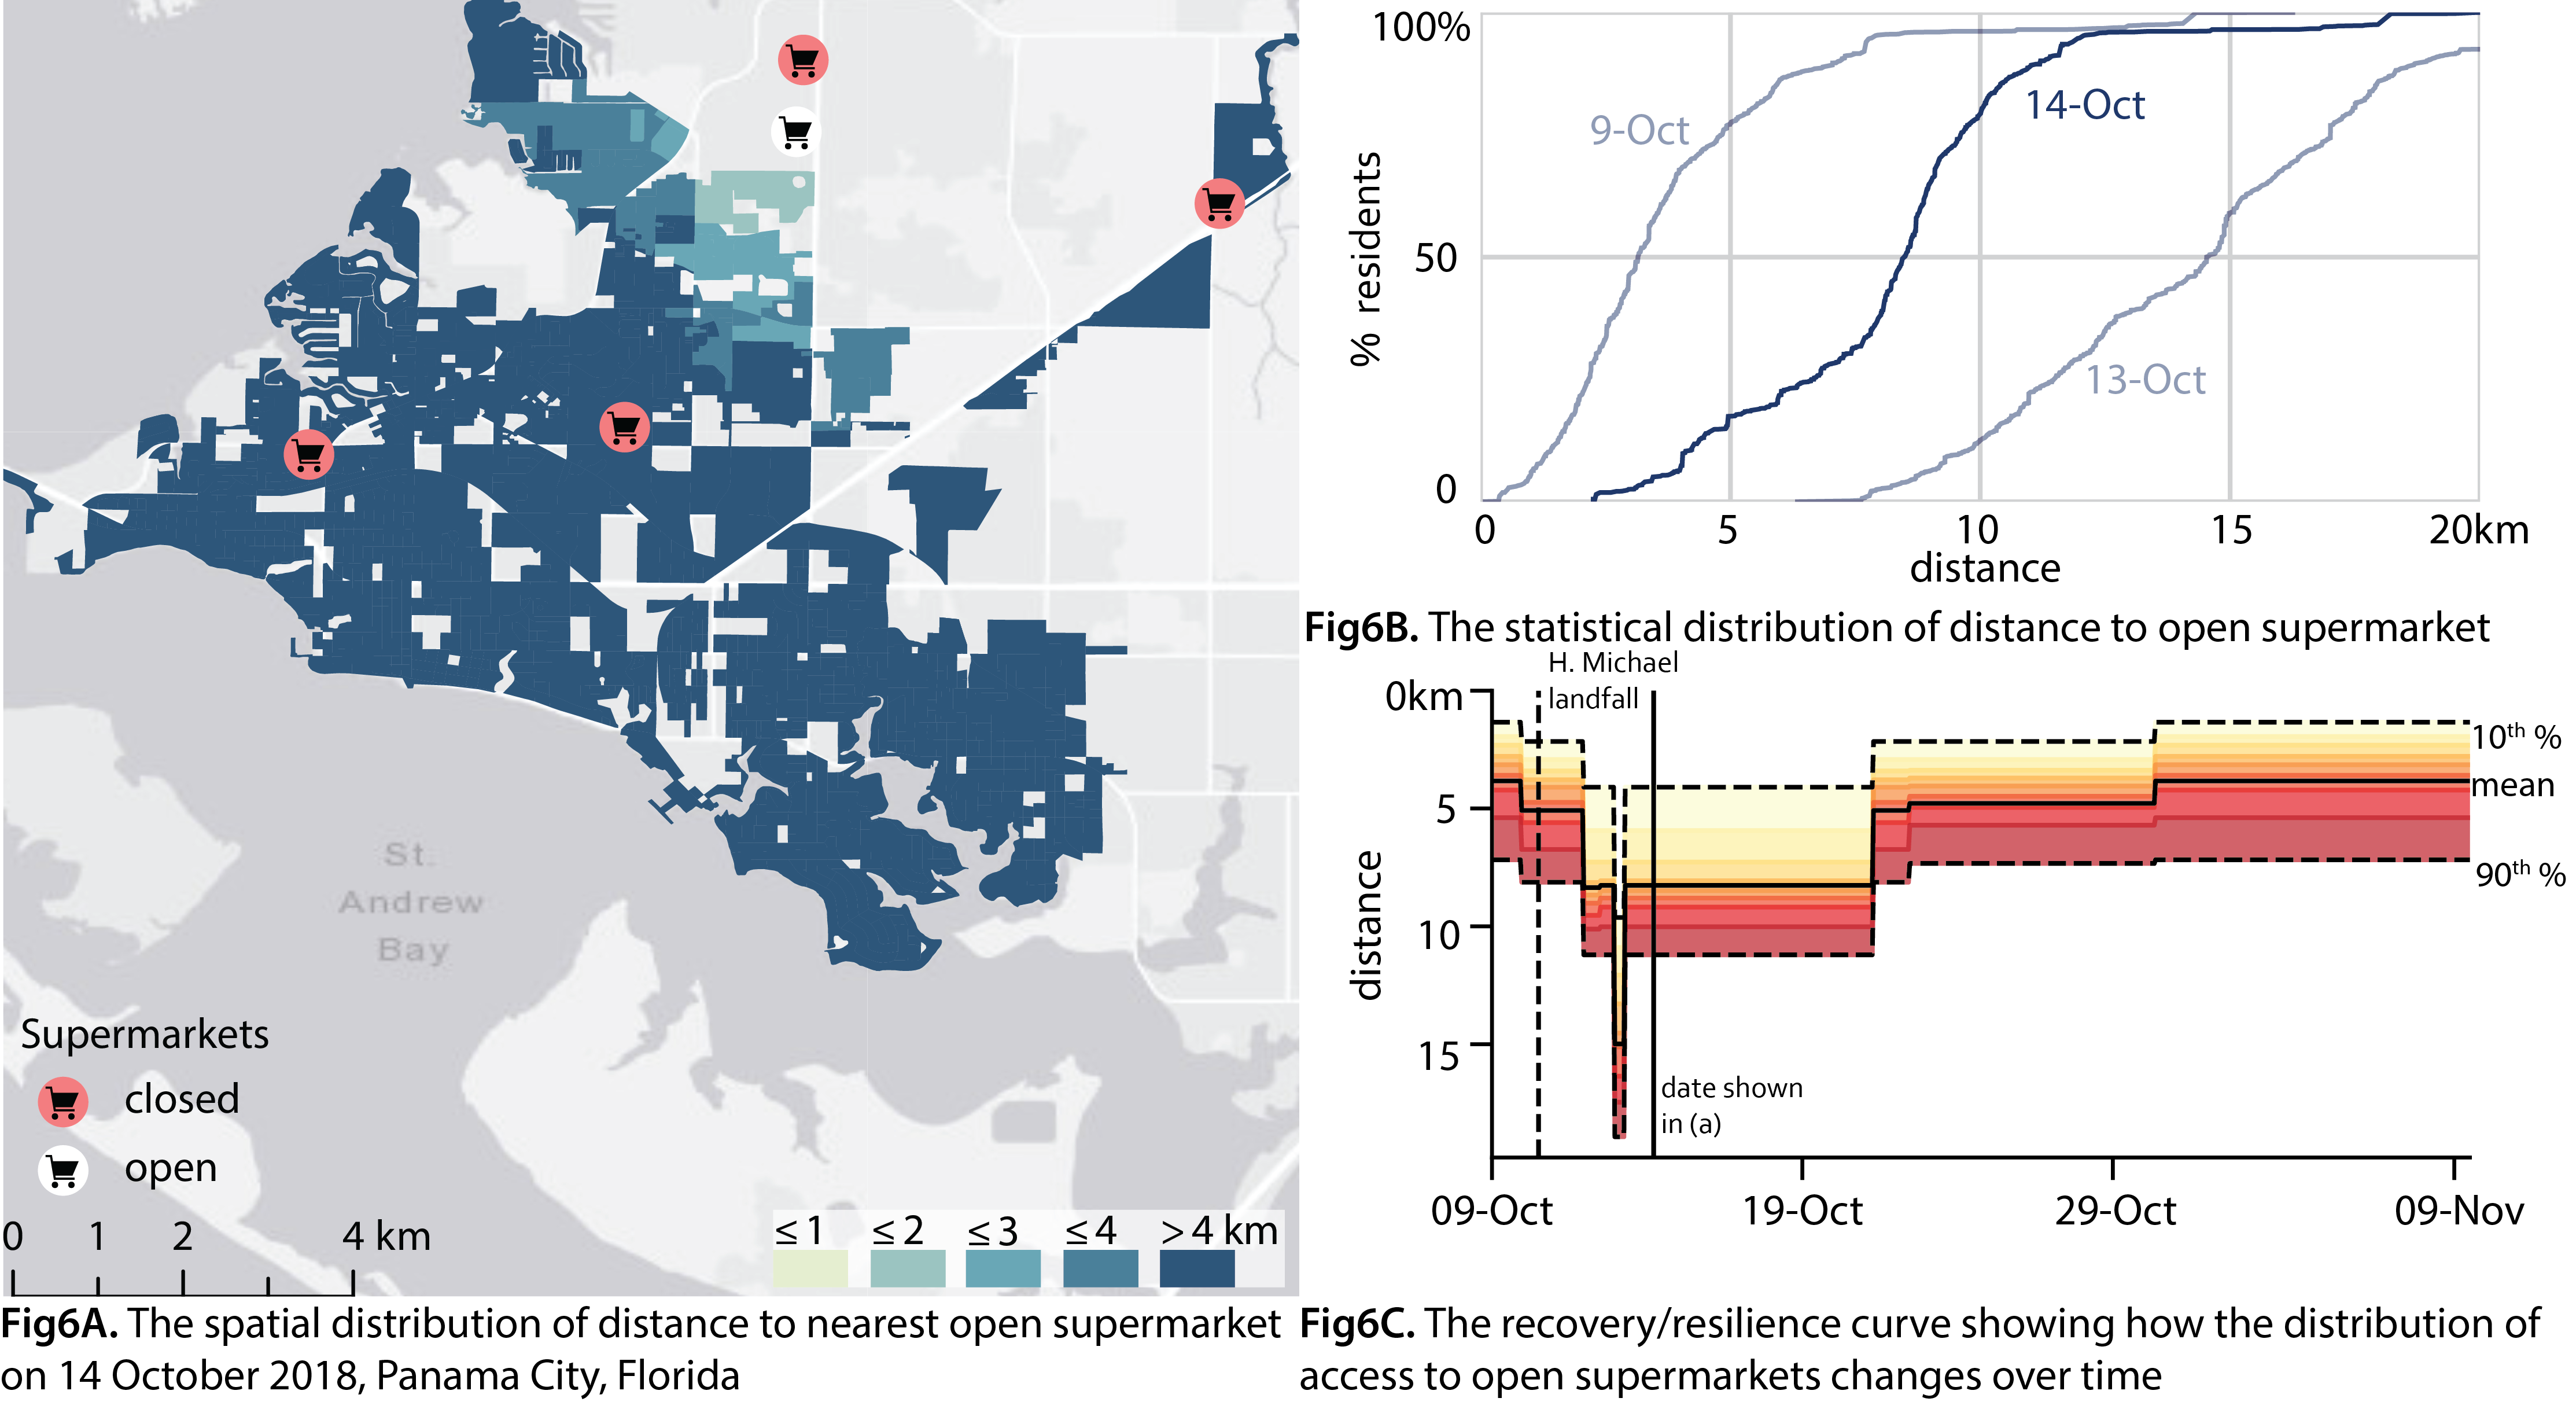
\includegraphics[width=\linewidth]{report/fig/FL_supermarket_resilience.png}
    \caption{The EAE approach to resilience considering supermarkets in Panama City, FL affected by Hurricane Michael.
    }
    \label{fig:FL_resil_super}
\end{figure*}
\begin{figure*}
    \centering
    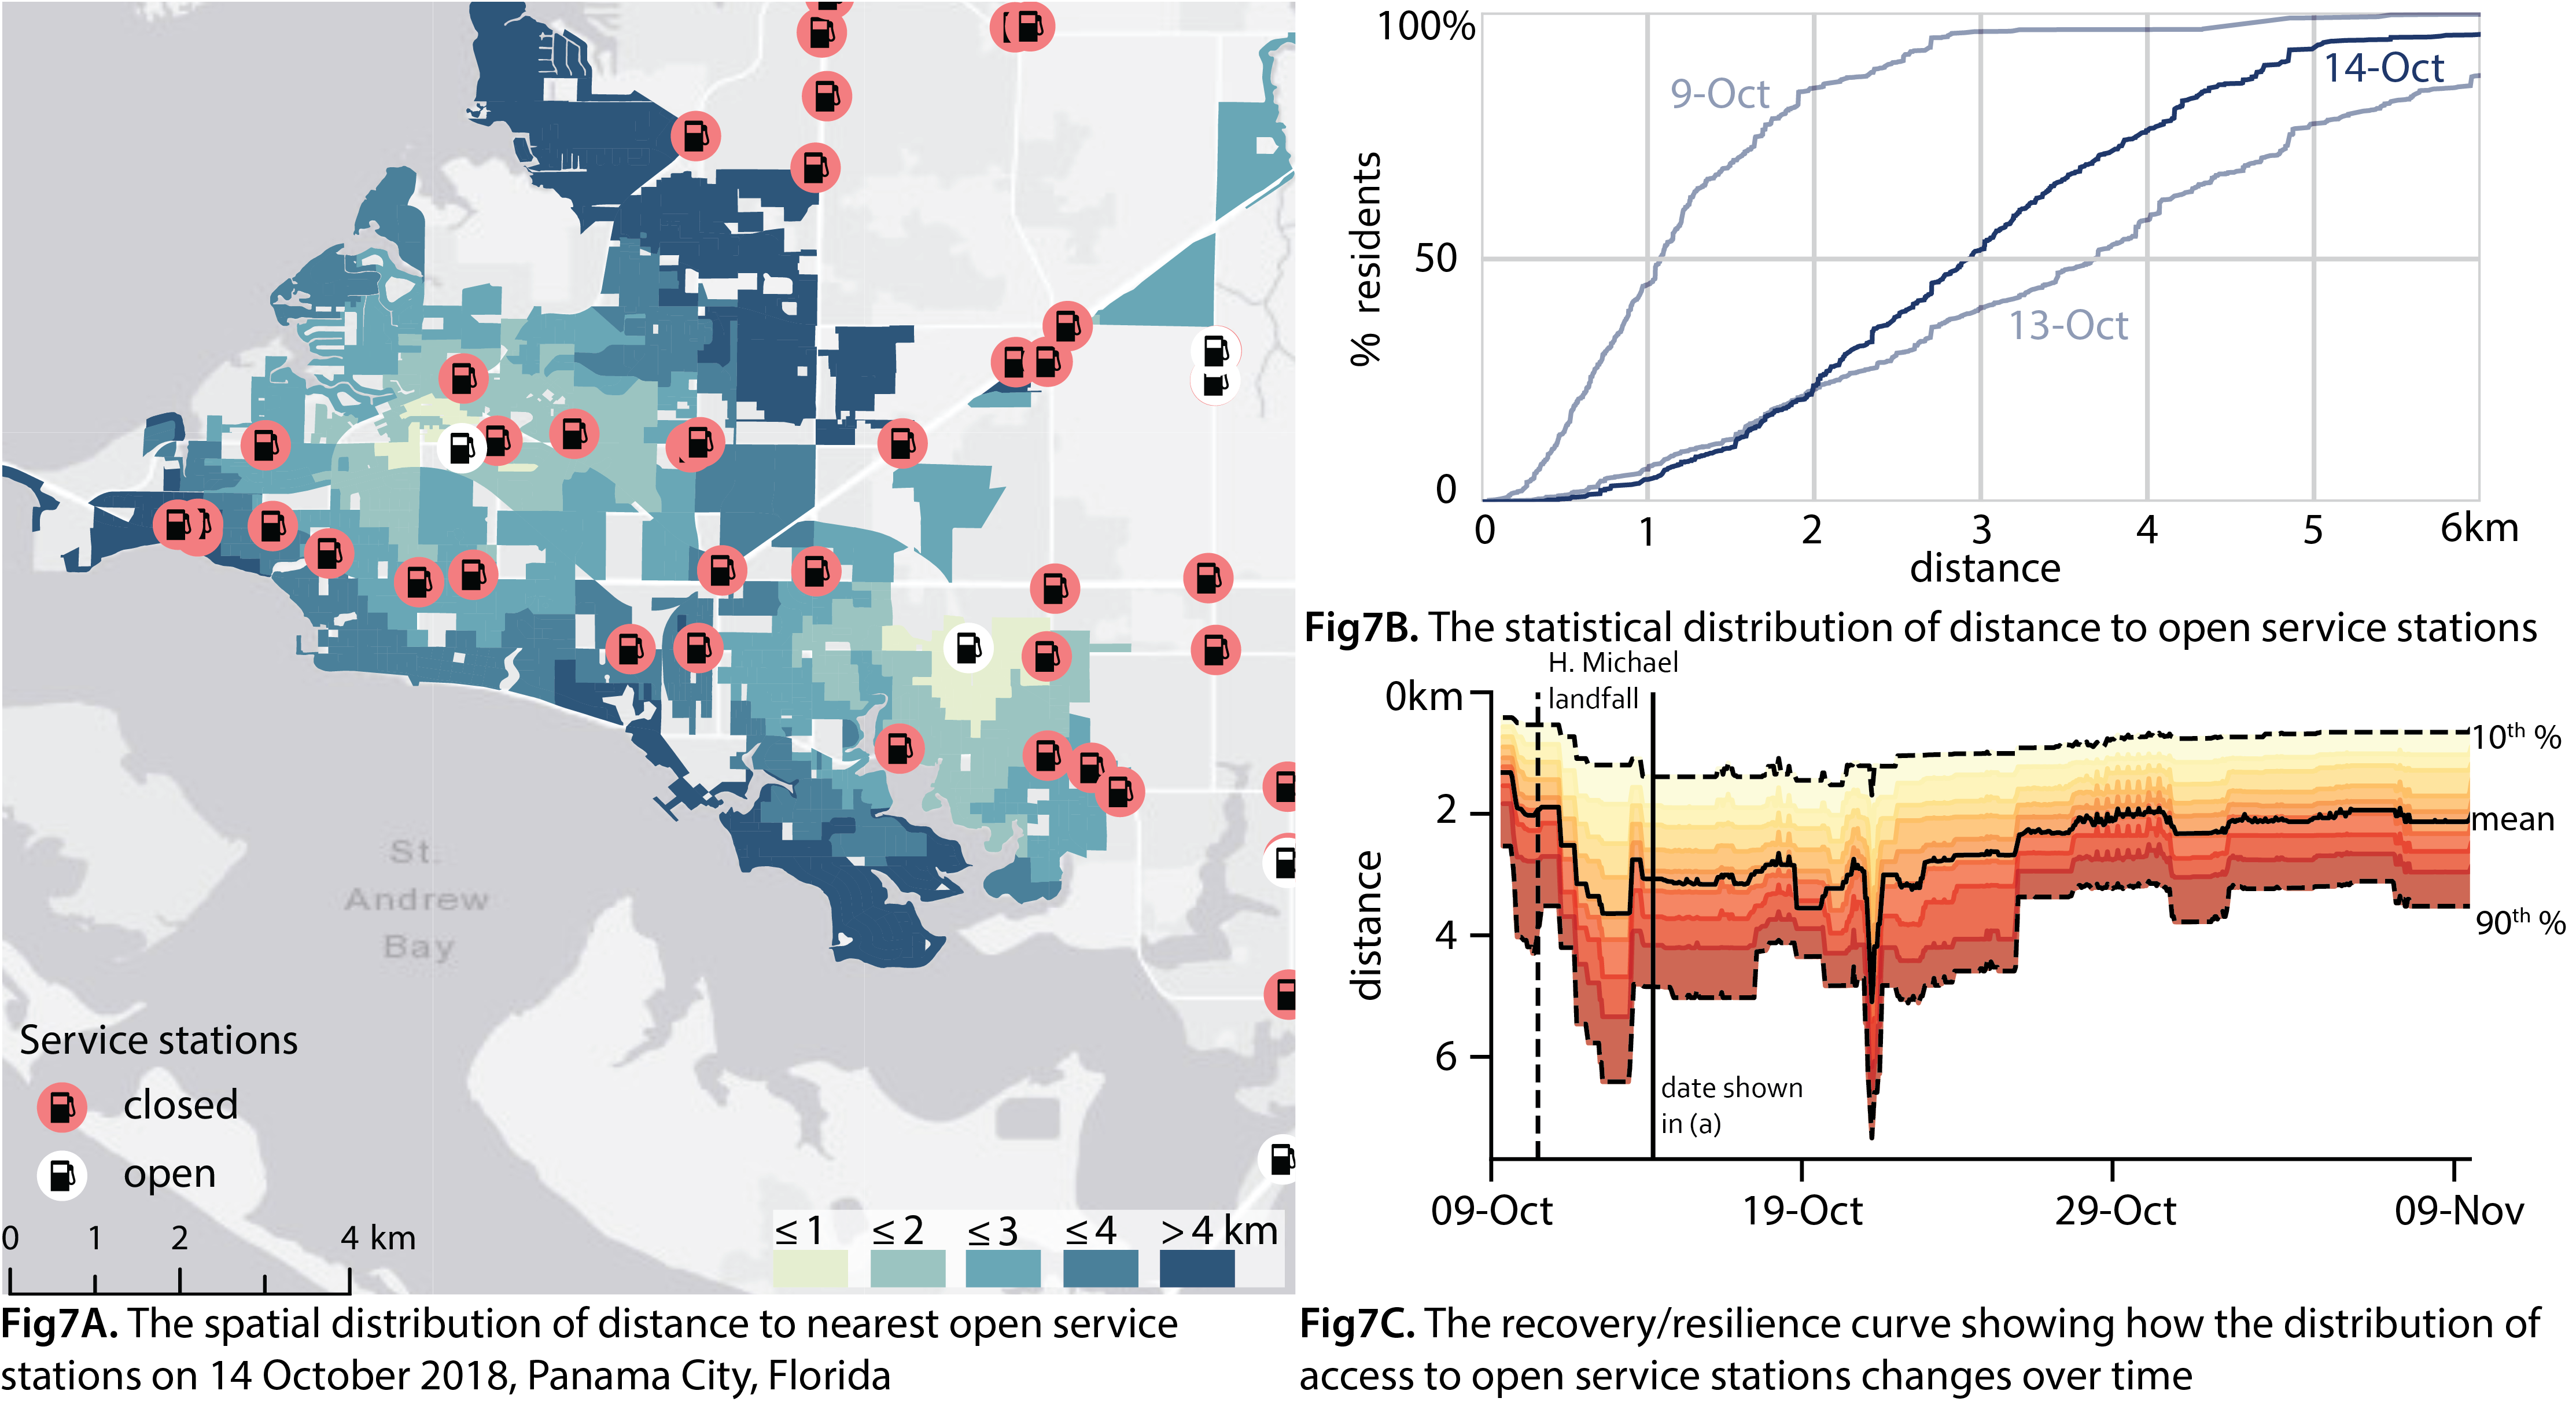
\includegraphics[width=\linewidth]{report/fig/FL_gasstation_resilience.png}
    \caption{The EAE approach to resilience considering service stations in Panama City, FL affected by Hurricane Michael.
    }
    \label{fig:FL_resil_gas}
\end{figure*}

\subsection{Community engagement and implementation}
With this illustrative example, we focused on demonstrating how steps 2-4 of the Equitable Access to Essential services (EAE) approach to resilience could be implemented. 
We focus on these steps as they are unique from other approaches to resilience.
In saying that, it is essential to appreciate the importance of community engagement and partnership (step 1) and, naturally, the step of implementing to build resilience (step 5).

Partnering and engaging with communities is the subject of many studies beyond risk and resilience assessment.
Building these relationships with communities and mana whenua (the indigenous people with traditional authority over the land) requires significant time and consideration.
For EAE, community knowledge and preference is essential when determining the important amenities and their distances; it may be that there are differing acceptable distances that vary not only between the amenities, but also across a region.
Given these various amenities and distances, understanding the relative importance of each requires approaches such as multicriteria decision analysis (e.g., \citeA{Guikema1999-aj}).

Evaluating access and equity is a dynamic and continuous process that should be done with any new development and population change within the community. 
During a hazard, it should be applied throughout the hazard cycle depending on the level of information and computational power available, but it should not be limited to the occurrence of hazards if we are to truly build community cohesion and sustainability.
Ideally communities would regularly evaluate access and access equality, and therefore evaluate how its community's resilience improves over time; this is possible given we can frequently and relatively easily update the location of amenities and evaluate the distance to the nearest ones. 
By incorporating demographic differences this enables us to evaluate the equality of changes.

Inclusion in these processes is essential for ensuring equality and equity.
To achieve this, it is important to be aware that cultural factors play a role in the acceptance of not only the interventions, but also the processes \cite{Flynn2018-mj}.
This highlights the importance of including indigenous peoples and m\=atauranga (indigenous knowledge, cultural values, and world view) --- an emerging area of research in the risk community (e.g., \citeA{Hikuroa2017-zf,Genuis2015-bq,King2007-zf})
Participatory scenario planning, is a useful approach for this and for dealing with the vast uncertainties, and it enables enables communities to explore potential futures and consider how best to respond \cite{Flynn2018-mj,Goodspeed2020-gm}.
Ultimately, by partnering with decision-makers, this approach will support land-use planning and both guide future development that is less exposed to nature's hazards, and foster more equitable and accessible communities. 


\section{Summary}
\label{sec:disc}
Understanding how to build community resilience has been described as one of today's most impactful research questions and practical challenges \cite{Caldarice2019-tv} and is urgently needed.
While there is significant work on resilience, the existing approaches are limited in the actionable insight they provide.

To address this need, we propose the equitable access to essentials (EAE) concept for community resilience.
This framing integrates key aspects of the traditional approaches to resilience and complements their use with the goal of maintaining, restoring, and improving equitable access to everyday amenities such as food, health care, and education, which are vital for residents to participate in life.
We outline a methodology along with an illustration of using EAE; however, although we recognize the fundamental importance of community partnership and subsequent action, we do not demonstrate those steps.
Our contribution is the proposal of the concept itself, and having it academically discussed and reviewed is an important and ethical step before applying it with a community. 

An EAE approach to resilience could provide a spatially explicit and hazard-general approach to quantifying resilience of access to services with a direct focus on people's well-being. 
Such an approach involves measuring the access of residents to the services and monitoring how that access changes before, during, and after a hazard event. 
Critical to our approach is the ability to discern how access changes between different demographics and vulnerable groups within a community to ensure equity.
Equally important is that we have devised the framework in a way that promotes continuous improvement of access to all residents and transforms the system, rather than bouncing back to pre-event conditions.
EAE can inform decision-making during all phases of the hazard cycle by providing actionable information from preparation to post-event improvement.
By being spatially explicit, EAE integrates resilience quantification with urban planning, which is crucial for our society's response to evolving threats exacerbated by climate change.

To end-users, we reiterate that while this approach is adaptable and scalable, resilience is place-based and therefore community specific, so an application of this methodology must include community engagement and understanding.

Reframing resilience as access to essential services promotes bounding forward, rather than bouncing back. 
It complements and integrates aspects of both dominant existing approaches to assessing community resilience. 
We encourage transformation by shifting the focus from the state of infrastructure to the value it provides to people. 
This, and the inclusion of vulnerability indicators, promotes addressing inequality, therefore building social sustainability and adaptive capacity of the community.
The EAE approach to resilience ultimately, and crucially, enables and encourages communities to build their resilience equitably. 

\backmatter

\section*{Acknowledgment}
TML conducted the majority of this research as a graduate student at the University of Michigan with the support of a Rackham PreDoctoral Fellowship.
We would also like to recognize support from the US National Science Foundation (grant 1638197) and One Concern Inc. (through a grant to the University of Michigan). 
Thank you to S. Meerow, T. Williams, T. Swanson, and the anonymous reviewers for their time and valuable suggestions when reviewing the manuscript.
Additionally, we acknowledge the editorial assistance of K Miller. 
All opinions expressed in this paper are our own.

\printbibliography

\appendix
\renewcommand\thefigure{A.\arabic{figure}} 

\section{}
\subsection{Technical guide}
\noindent Code is available at \url{https://github.com/tommlogan/access_to_essentials}.


Tools to conduct this analysis are becoming increasingly user-friendly (e.g. \citeA{noel2019-pypi}), but currently coding ability is required. This technical appendix outlines the approach, tools, and steps:

\begin{enumerate}[listparindent=0em, parsep=0.5em,itemindent=0em]
    \item Regional data

    One of the first steps is to acquire the geographic data for the region of interest. 
    You need to decide the spatial resolution at which to conduct the analysis. 
    Here, we use the census block level (generally equivalent in size to a city block) however this could also be conducted at the parcel or block group level. 
    The tradeoff is the computational burden and the accuracy.
    Also, using larger spatial areas risks overlooking vulnerable populations \cite{Logan2017-fr}.
    Shapefiles for the USA can be downloaded from \cite{Manson2018-ug}.
    Demographic data that can be joined to the shapefiles is available from \citeA{Manson2018-ug} or \citeA{US_Census_Bureau2017-ti}.
    
    \item Service/facility/amenity locations
    
    The geo-location of all facilities is needed for the analysis.
    These are often available from open-data portals hosted by the city or OpenStreetMap (OSM).
    For example, the services used in Fig. \ref{fig:bal_services} were retrieved from the following locations:
    \begin{itemize}
        \item \textit{Schools, libraries, and hospitals}: \url{https://data.baltimorecity.gov/dataset}
        \item \textit{Supermarkets}: \url{https://overpass-turbo.eu/} using the ``shop=supermarket" key. This data can be downloaded as a .kml file.
    \end{itemize}
    
    \item Routing/Network distance
    
    We now require the network distance from all origins to destinations.
    The approach we use is described in \cite{Logan2017-fr}.
    We use OpenStreetMap (OSM) data and the Open Source Routing Machine (OSRM) \cite{luxen-vetter-2011} (\url{http://project-osrm.org/}) running via Docker \cite{Merkel2014-op} on a local server.
    However, there are other routing algorithm options that are improving the computational speed, such as \citeA{noel2019-pypi}.
    Instructions to set-up an OSRM server are available online, for example: \url{https://reckoningrisk.com/coding/2017/OSRM-server/}.
    A more user-friendly approach is to install `Docker' (essentially a virtual environment) on your computer and pull (download) an OSRM server that has already been setup: \url{https://hub.docker.com/r/osrm/osrm-backend/}.
    
    \item Nearest service through time
    
    Access is currently specified as being the distance to the \textit{nearest} service (although this can and should be enhanced). 
    Therefore, each city block is assigned the distance to each of the nearest types of service.
    To understand how access changes through time, the facilities need to be assigned an indicator for whether it is operating.
    For any point in time then, the distance from each block to the service is the distance to the nearest operating service.
    
    \item Graphical and statistical output
    
    The paper uses Python and ArcGIS Pro to construct the figures and maps. 
    The code for the plotting in Python is provided in the Github repository: \url{https://github.com/tommlogan/access_to_essentials}.
    The ECDF's are explained in \cite{Logan2017-fr}.
    
\end{enumerate}

\clearpage
\subsection{Acceptable Access}

\begin{figure*}[h]
    \centering
    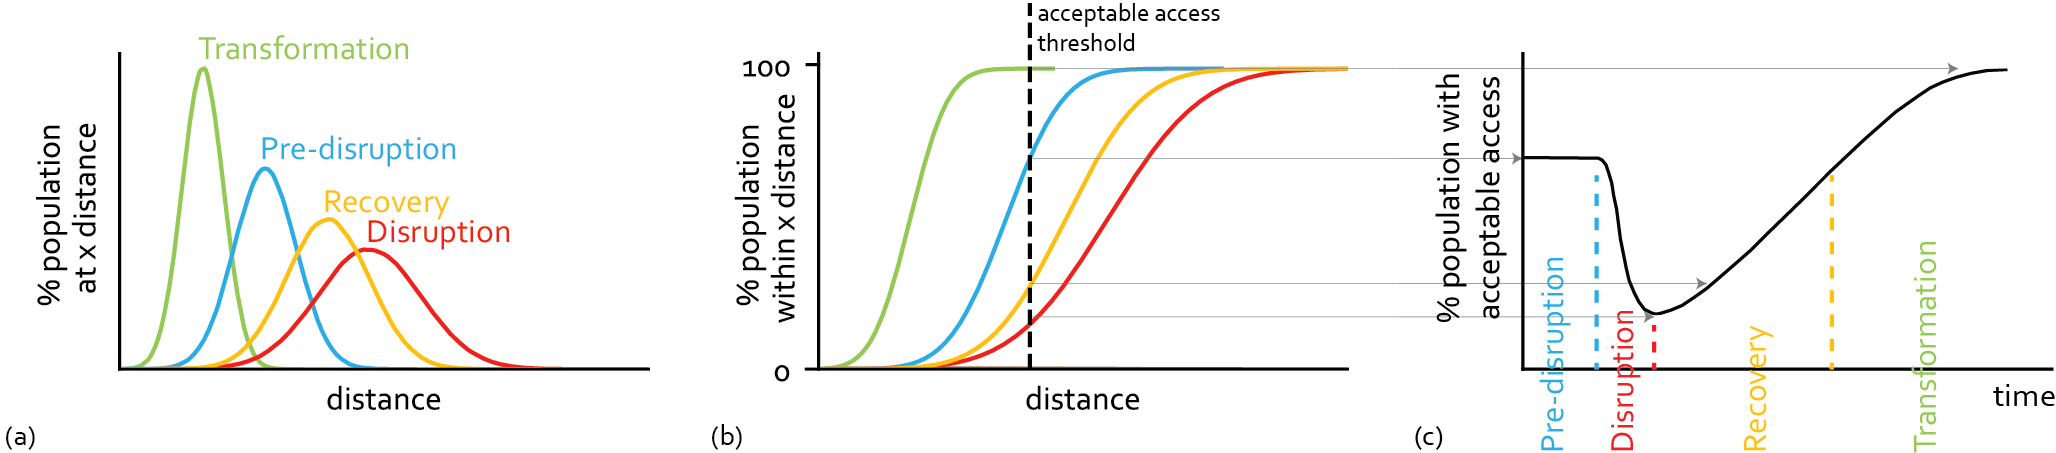
\includegraphics[width=\linewidth]{report/fig/dist_to_resil.png}
    \caption{
    How the distribution of access maps onto the resilience function (aka recovery curve). (a) these are the density functions (idealized histograms) of the distance of residents to their nearest service.
    Each distribution curve represents a different phase of the hazard cycle. 
    (b) these cumulative distribution functions are variants of (a) and show the percentage of the population that live less than the distance on the $x$ axis.
    The threshold of acceptable access is shown here. Where this line intersects with the CDFs we can identify what percentage of the population has acceptable access.
    (c) mapping these values onto their associated time results in this figure that shows acceptable access changing with time, and is a recovery curve.
    }
    \label{figS:cdf_to_res}
\end{figure*}

\begin{figure}[h]
    \centering
    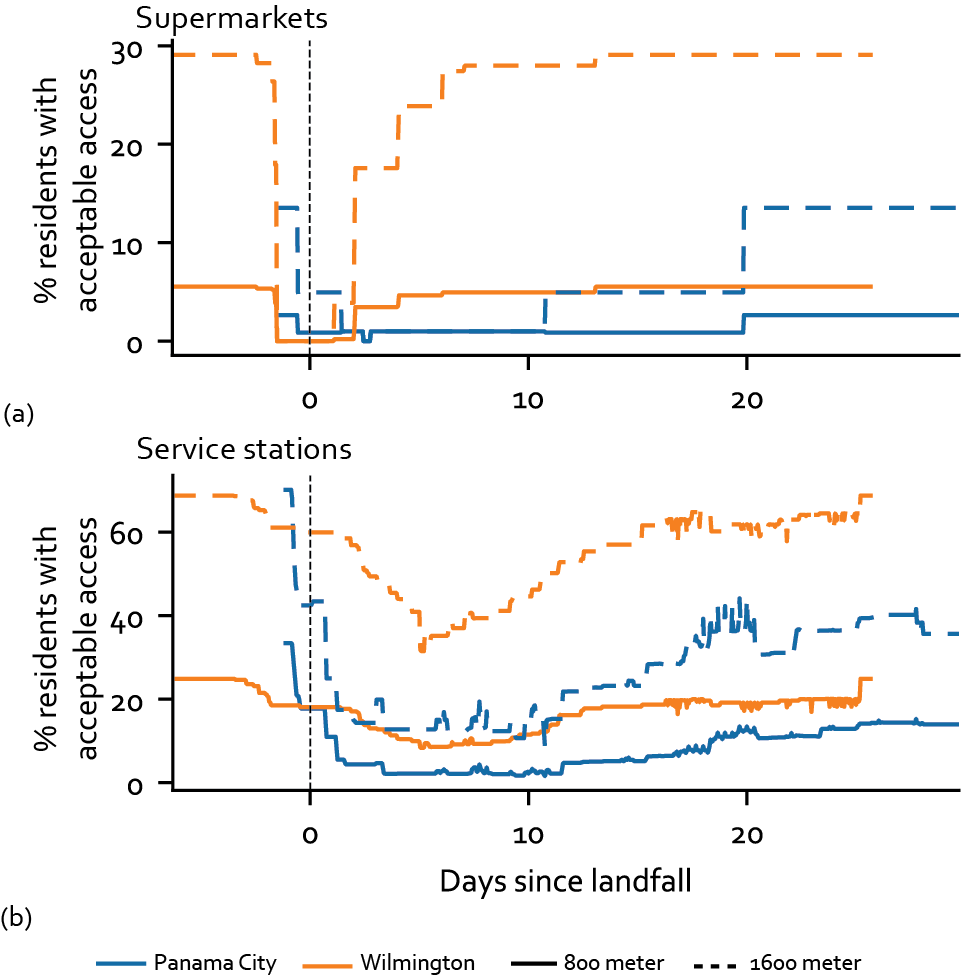
\includegraphics[width=0.5\linewidth]{report/fig/sufficient_only.png}
    \caption{The recovery curves, for Panama City following Michael and Wilmington following Florence, showing the percentage of residents in each city with acceptable access to both (a) supermarkets and (b) service stations. Acceptable access is defined by two distance thresholds. 
    }
    \label{fig:threshold}
\end{figure}



\end{document}


